\documentclass[11pt]{article}

\usepackage[margin=1.05in]{geometry}
\usepackage{amsmath,amssymb,amsthm}
\usepackage{mathtools}
\usepackage{graphicx}
\usepackage{booktabs}
\usepackage{array}
\usepackage{microtype}
\usepackage{xcolor}
\usepackage[shortlabels]{enumitem}
\usepackage[colorlinks=true,linkcolor=blue!45!black,citecolor=blue!45!black,urlcolor=blue!45!black]{hyperref}
\hypersetup{pdftitle={Endpoint crossings for random walks with heavy-tailed runs and for aging walks},pdfauthor={Arjun Pemmasani}}

% ---------- theorem environments ----------
\newtheorem{theorem}{Theorem}[section]
\newtheorem{lemma}[theorem]{Lemma}
\newtheorem{proposition}[theorem]{Proposition}
\newtheorem{corollary}[theorem]{Corollary}
\newtheorem{conjecture}[theorem]{Conjecture}
\theoremstyle{definition}
\newtheorem{definition}[theorem]{Definition}
\newtheorem{example}[theorem]{Example}
\theoremstyle{remark}
\newtheorem{remark}[theorem]{Remark}

% ---------- notation macros ----------
\newcommand{\Z}{\mathbb{Z}}
\newcommand{\E}{\mathbb{E}}
\newcommand{\Prob}{\mathbb{P}}
\newcommand{\Var}{\operatorname{Var}}
\newcommand{\CP}{\mathrm{CP}}

\title{Endpoint crossings for random walks with heavy-tailed runs\\ and for aging walks}
\author{Arjun Pemmasani\\[2pt]
\small Department of Mathematics, Harvey Mudd College\\
\small Claremont, CA 91711, USA\\
\small \texttt{apemmasani@hmc.edu}}
\date{}
\begin{document}
\maketitle

\begin{abstract}
Consider a random walk on $\Z$ whose direction is an alternating renewal
process started in equilibrium, with independent run lengths of tail
$k^{-\alpha}$, $1<\alpha<2$. This is a lattice analogue of a L\'evy walk. We
compare the probability of each end, $\pm N$, after $N$ steps with that of
the middle. Wang, Li and H\"anggi observed, as a heuristic for heat
conduction, that the ends and the middle decay at the same rate when $\alpha$
is the golden ratio. We prove the lattice form of their observation, with its
constant. Namely, the ends beat the middle for large $N$ exactly when $\alpha$
is below the golden ratio. We also study an aging walk, which switches at
step $k$ with probability $c/k$. With a fixed first step each interior
position ties with the end exactly at $c=1$, for every $N$. We prove the same
for an aging walk with $d$ states, whose vector of counts is exactly uniform
at the tie.
\end{abstract}

\medskip
\noindent\textbf{Keywords:} persistent random walk; alternating renewal process; heavy tails;
L\'evy walk; golden ratio; aging random walk; P\'olya urn.

\noindent\textbf{MSC2020:} 60G50; 60K05; 60F05; 60J10; 60C05; 82C41; 82C70.

\section{Introduction}\label{sec:intro}

A lattice L\'evy walk moves on $\Z$ in runs of alternating direction. The
run lengths are independent, and their tails are regularly varying with an
index $\alpha$ between $1$ and $2$, so a run has a finite mean and an
infinite variance. Let $A_N$ be the number of right steps among the first
$N$. The position of the walk after $N$ steps is $2A_N-N$, so the law
$P_N(k)=\Prob(A_N=k)$ on $\{0,\dots,N\}$ is the law of the walk read on its
natural lattice. L\'evy walks are a standard model of
superdiffusion~\cite{zdk2015}, and the same walk describes heat transport in
one-dimensional lattices~\cite{dsd2013,wlh2016} and the occupation time of an
alternating renewal process~\cite{godrecheluck2001,lamperti1958}. Its
profile has a central peak and two ballistic side
peaks~\cite{zdh2011,dzh2012}, and the physics literature describes the part
between them by an infinite density~\cite{rdhb2014,rdhb2014b}. We describe
$P_N(k)$ for every $k$, with proofs, with one exception that we state below.

\subsection{The picture}\label{sec:intro-picture}

Figure~\ref{fig:atlas} shows $P_N$ for $N=5000$ on a logarithmic scale.
Four pieces make up the row. We call the right steps plus slots.
\begin{itemize}[nosep]
\item The bulk. Near $pN$, where $p$ is the long-run fraction of plus
slots, the law is a stable density at the scale $B_N$ of the larger of the
two run-length fluctuations. Here $B_N$ grows like $N^{1/\alpha_*}$ up to a
slowly varying factor, with $\alpha_*$ the smaller index.
\item The big-jump zones. A count $k$ with $k-pN$ much larger than $B_N$
needs one plus run of macroscopic length, a giant run, and the law of that run
gives the bin its size, which is of order $T_\plus(N)$ on the ballistic range,
with $T_\plus$ the tail of a plus run. The giant run is either complete and lies
in the interior or the final run, censored at slot $N$, and the bin is the sum
of the two contributions.
\item The boundary layers. At $k=N-j$ with $j$ fixed, the giant run is the
final one, and the only question is where it started. It starts right after the $j$-th minus slot exactly when a
minus run ends there, so the layer is $T_\plus(N)$ times the renewal mass
function $u_\minus(j)$ of the minus runs.
\item The atoms. The bin $k=N$ is the event that the first run covers the
row, and its mass is the tail of the first run.
\end{itemize}
The first run is the preparation of the walk. It may be a fresh run, a run
seen from a typical time, or anything else, and it enters each of the four
pieces through its own criterion.

\begin{figure}[t]
\centering
\includegraphics[width=\textwidth]{atlas}
\caption{(a) The law $P_N(k)$ for $N=5000$, run lengths with
$f(n)\propto n^{-5/2}$ for both signs and a fresh plus start, on a
logarithmic scale, with the four pieces of Theorems~\ref{thm:bulk}
and~\ref{thm:bigjump}. The two ends of the horizontal axis are stretched.
(b) The position $j^*_N$ of the interior minimum near the plus end against
$N$, on logarithmic axes, with the law of Theorem~\ref{thm:antimode} and the
refined prediction with $C(j)$ from Theorem~\ref{thm:second-order}.
Section~\ref{sec:verify} describes the computations.}
\label{fig:atlas}
\end{figure}

\subsection{Results}\label{sec:intro-results}

We state the hypotheses in Section~\ref{sec:hypotheses}. They are regular
variation of the two tails with indices in $(1,2)$, written (RV), the local
form $f_\sgn(n)\sim\alpha_\sgn T_\sgn(n)/n$ of the mass functions, written
(LR), and aperiodicity, written (SPAN). The run laws may differ between the
two signs, so the two stable scales $b_{\plus,N}$ and $b_{\minus,N}$ may
differ, and their ratio may oscillate. Every theorem below holds for every
relation between the two scales. When the smaller scale is smaller than the
other by an unbounded factor, one window on the side of the sign with the
smaller scale is described only in part, as we say below. When the ratio of
the scales stays bounded, Theorem A covers that window. The model is
symmetric, so the side in question is the plus side when the plus scale is the
smaller one and the minus side otherwise. We write $s$ for the sum of the two mean run lengths and $p$
for the fraction of the plus mean.

\emph{The bulk.} Theorem~\ref{thm:bulk} says that for a fresh start, under
(RV) and (SPAN),
\[
 \sup_{k\in\Z}\bigl|B_NP_N(k)-h_N\bigl((k-pN)/B_N\bigr)\bigr|\to0,
 \qquad \sup_kP_N(k)\le\frac C{B_N},
\]
where $h_N$ is the density of $(1-p)\theta_{\plus,N}Z_\plus-p\,\theta_{\minus,N}Z_\minus$,
with $Z_\pm$ independent totally skewed stable variables. The supremum runs
over the whole row. On a window $|k-pN|\le KB_N$ the local limit also follows
from a strong renewal theorem of Berger, and what is new is the uniformity over
every bin under (RV) and (SPAN) alone. Outside the bulk the theorem says only that
every bin is
$o(1/B_N)$, and the next theorem says what the bins are.

\emph{Big jumps and the boundary layer.} Put $L_k=(k-pN)/(1-p)$, the length
of the plus run that carries a typical configuration to the count $k$.
Theorem~\ref{thm:bigjump} says that for a fresh plus start, under (RV) and
(SPAN) for both signs and (LR) for the plus sign,
\[
 P_N(k)=\Bigl[\gamma(N-k)\,f_\plus(\lfloor L_k\rfloor)+T_\plus(\lfloor L_k\rfloor)\,u_\minus(N-k)\Bigr](1+o(1))
\]
uniformly on $pN+K\lambda_NB_N\le k\le N$, in the sense that the error
tends to zero as $N\to\infty$ and then $K\to\infty$. Here $\gamma(j)$ is an
explicit finite sum with $\gamma(j)\sim js/\mu_\minus^2$, and
$\lambda_N=1+\log(B_N/b_{\plus,N})$, which equals $1$ when the plus scale is the
larger one. The first term is a complete giant
run and the second a censored final run. At $k=N-j$ with $j$ fixed the
theorem reduces to $P_N(N-j)/T_\plus(N)\to u_\minus(j)$, which needs only (RV)
for the plus sign. As $j$ grows, $u_\minus(j)\to1/\mu_\minus$ and the layer
joins the big-jump zone continuously. The junction with the bulk holds only
in the double limit. Remark~\ref{rem:no-single-formula} shows that neither
the bulk profile nor the big-jump kernel nor their sum approximates $P_N$
with relative error $o(1)$ over the plus side. When the plus scale is the
smaller one, on the window $KB_N\le k-pN\le K\lambda_NB_N$ we prove only the
bulk estimate and the lower bound $P_N(k)\ge(1-o(1))G_N(k)$, with $G_N$ the
bracket above, and we do not describe $P_N$ there. When the minus scale is the
smaller one the mirror window appears at the minus end. (LR) suffices for the
theorem, and Example~\ref{ex:rv-not-lr} shows that (RV) alone does not, since
the kernel reads $f_\plus$ at a single point. Whether some local condition
strictly weaker than (LR) suffices is open (Remark~\ref{rem:wr}). Read
at $k=vN$ the theorem gives the infinite density
\[
 \frac{P_N(\lfloor vN\rfloor)}{T_\plus(N)}\to
 \frac1{\mu_\minus}\Bigl[\alpha_\plus(1-\ell)\ell^{-\alpha_\plus-1}+\ell^{-\alpha_\plus}\Bigr],
 \qquad \ell=\frac{v-p}{1-p},
\]
with its censored-run term (Corollary~\ref{cor:infinite-density}).

\emph{Preparation.} Theorem~\ref{thm:preparation} describes every
preparation through the first-run decomposition of
Proposition~\ref{prop:first-run}. Write $\nu_\sgn(n)$ for the probability
that the first run has sign $\sgn$ and length $n$, and $Q_\sgn(n)$ for the
probability that it has sign $\sgn$ and length at least $n$. On every
macroscopic interior of the row the bulk approximation holds with no condition
on the preparation. It holds uniformly over $1\le k<N$ exactly when
$B_n(\nu_\plus(n)+\nu_\minus(n))\to0$, which we call the bulk criterion. The
preparation is invisible in the
boundary layer at the plus end exactly when $\nu_\plus(n)=o(T_\plus(n))$. On the
big-jump zone up to the end the same condition is sharp, while on its interior
only window averages of $\nu_\plus$ matter, and the window condition is sharp
under (LR) for both signs. At the plus end the conditions are nested,
since $Q_\plus(n)=o(T_\plus(n))$ implies $\nu_\plus(n)=o(T_\plus(n))$, which
implies $B_n\nu_\plus(n)\to0$, the plus half of the bulk criterion. When a
condition fails the theorem gives the exact correction, as a directional
defect in the bulk, and as an additive term in the big-jump zone and at the
end. The stationary preparation, which is
the equilibrated start of the physics literature, satisfies the bulk
criterion and fails the other two, and Corollary~\ref{cor:stationary} gives
its corrections in closed form. Corollary~\ref{cor:no-trim} shows that no
trimming of the row by $o(N)$ bins removes the dependence on the
preparation for every preparation at once.

\emph{The shape.} Theorem~\ref{thm:mode} compares the endpoint atoms with
the bulk for a preparation that satisfies the bulk criterion. An endpoint is
the global mode when its atom exceeds $H_N/B_N$ by a fixed factor, with $H_N$
the height of the profile, and the bulk wins when both atoms are smaller by a
fixed factor. For the stationary preparation
with equal indices this is the golden ratio threshold. The endpoints win for
$\alpha<\varphi=(1+\sqrt5)/2$, the bulk wins for $\alpha>\varphi$, and at
$\alpha=\varphi$ with pure power tails the bulk wins by the explicit factor
$1/\mathcal C(\varphi)=1.288\ldots$, with $\mathcal C$ as in~\eqref{eq:Calpha}.

Theorem~\ref{thm:antimode} locates the interior minimum between the bulk and
the plus end for a fresh plus start. Suppose that $u_\minus(j)>1/\mu_\minus$
for every $j\ge1$. This holds for every strictly log-convex law of the minus
runs. Then the minimum sits at $N-j^*_N$ with
\[
 T_\minus(j^*_N)\sim\frac{2\alpha_\plus s}N .
\]
So $j^*_N$ grows like the stable scale of the minus runs. At finite $N$ the
minimizer of $u_\minus(j)+C(j)/N$ predicts $j^*_N$ better, and $j^*_N$ is
asymptotic to it. Here $C(j)$ is the exact second-order coefficient of
Theorem~\ref{thm:second-order}. When $u_\minus$ dips below its limit the
minimum stays at bounded distance from the end. These results compare bins in
different zones. They do not say that the law is monotone between the
extrema, and the number of local extrema inside the layers is not determined
here.

\emph{Identification.} Proposition~\ref{thm:inverse} reads the run laws off the
ends. For a fresh plus start the atoms give the law of the plus runs directly,
since $P_N(N)=T_\plus(N)$. The law of the minus runs comes from the boundary
layer, since $P_N(N-j)/P_N(N)\to u_\minus(j)$ and the renewal equation inverts
$u_\minus$. The minus end cannot replace the atoms. Its ratios determine a
renewal mass function only up to a geometric thinning of the run law, and the
normalization of the law does not remove this freedom
(Remark~\ref{rem:thinning}).

\subsection{Related work}\label{sec:intro-related}

\emph{Infinite densities and big jumps.} Rebenshtok, Denisov, H\"anggi and
Barkai~\cite{rdhb2014,rdhb2014b} derived the infinite density of a L\'evy
walk from the Montroll and Weiss equation, formally and in continuous time.
For the two-state velocity model their density
\cite[Eqs.~(8) and~(10)]{rdhb2014} has the shape
$|v|^{-1-\alpha}[\alpha-(\alpha-1)|v|]$. A complete giant run alone would give
the linear term $-\alpha|v|$, and the censored final run adds $+|v|$, so their
formula already contains the censored run.
What is new in Corollary~\ref{cor:infinite-density} is a proof on the lattice
at fixed time, uniform up to the end, together with the boundary layer and the
preparation. In the physics model each flight chooses its direction
independently, and consecutive flights in the same direction merge into one
run. This gives the alternating walk with run laws thinned geometrically
with parameter $\frac12$, as in Remark~\ref{rem:thinning}. Vezzani, Barkai and
Burioni~\cite{vbb2019,vbb2020} derived the same tail from a single big jump.
Wang, Schulz, Deng and Barkai~\cite{wsdb2018} treat the occupation time of an
alternating renewal process with one law for both states and find a boundary
layer and an atom at the ends. They work in continuous time through a double
Laplace transform, with one law and a start of fair random sign, and they leave
the effect of the preparation on the rare fluctuations open. Here the layer is
proved on the lattice for two laws, uniformly up to $j=o(N)$, with a kernel
$\kappa$ that depends on the start (Theorem~\ref{thm:bigjump}(a) and~(c)).
Wang, H\"oll and Barkai~\cite{whb2020} treat the infinite-mean case.
Akimoto~\cite{akimoto2023} computes the moments of the occupation time for the
ordinary and the equilibrium start and shows that they differ for
$1<\alpha<2$. Theorem~\ref{thm:preparation} treats an arbitrary preparation bin by
bin and gives, for each zone, a sharp criterion for when the start is invisible
and the exact correction when it is not. The classical integral limit theorems for the sojourn time of an
alternating renewal process are due to Tak\'acs~\cite{takacs1957,takacs1959} and
Kesten~\cite{kesten1962}, and they are statements in distribution, while every
statement here concerns single bins. The
golden ratio appears in Wang, Li and H\"anggi~\cite{wlh2016} as the exponent
at which the side peaks and the central peak decay at the same rate, with the
edge exponent of Cipriani, Denisov and Politi~\cite{cdp2005}, and
Lee-Dadswell, Nickel and Gray~\cite{ldng2005} found the conduction exponent
$(3-\sqrt5)/2$ by a hydrodynamic argument. The threshold itself is the
exponent identity $\alpha-1=1/\alpha$. What Theorem~\ref{thm:mode} adds is the
comparison of single bins as a theorem and the constant $\mathcal C(\varphi)$.

\emph{Local limit theorems and renewal theory.} Doney~\cite{doney1991} proved
a bivariate local limit theorem in the stable domain, and
Berger~\cite{berger2019} proved multivariate local large deviations and strong
renewal theorems. His Theorem~3.3 applied to the walk of run lengths, together
with the fresh-plus identity of Proposition~\ref{prop:fresh-identity}, gives
the window $|k-pN|\le KB_N$ of Theorem~\ref{thm:bulk}, and Section~\ref{sec:bulk}
explains what the rest of the theorem adds and why it needs new work. Melbourne, P\`ene and Terhesiu~\cite{mpt2026} prove mixing local
limit theorems with multivariate stable limits on Young towers, which give one
bin at the stable scale with the first and the last run restricted to fixed
lengths. In the i.i.d.\ renewal setting Theorem~\ref{thm:bulk} removes these
restrictions. We use the local large deviation bound of Caravenna and
Doney~\cite{caravennadoney2019} (see also~\cite{melbourneterhesiu2022}) for sums
of a fixed number of variables. The local one-big-jump theorems for
sums of independent variables are due to Denisov, Dieker and
Shneer~\cite{dds2008} and Berger, Birkner and Yuan~\cite{bby2023}, and the one
under exactly the local condition (LR) is~\cite[Theorem~2.4]{berger2019ptrf}.
That theorem gives the probability that a fixed number of plus runs adds up to a
given large value. It does not give Theorem~\ref{thm:bigjump} directly, because
the number of runs before slot $N$ is random and tied to the run lengths, because
the big jump may be made by the final run, which the horizon cuts off and no
statement about complete sums sees, and because the kernel must hold uniformly up
to the endpoint, where only boundedly many minus slots remain. The proof of
Theorem~\ref{thm:bigjump} does not use these theorems. What is new there is
the occupation count at a fixed time, where a complete giant run enters with
the renewal density of its start and a censored run with the boundary kernel.
The second-order coefficient rests on the second-order renewal theorem of
Frenk~\cite{frenk1982}, see also Rogozin~\cite{rogozin1973} and
Doney~\cite{doney2023}, and the monotonicity of $u_\minus$ on de Bruijn and
Erd\H{o}s~\cite{debruijnerdos1953}.

\emph{The walk.} The walk is the directionally reinforced random walk of
Mauldin, Monticino and von Weizs\"acker~\cite{mmw1996}, with limit laws by
Horv\'ath and Shao~\cite{horvathshao1998}, and the persistent random walk of
C\'enac, Le Ny, de Loynes and Offret, who prove functional scaling limits,
a stable L\'evy process for $1<\alpha<2$~\cite{clnlo2018,clnlo2019}. Magdziarz,
Scheffler, Straka and \.Zebrowski~\cite{mssz2015} prove limit theorems for
L\'evy walks in continuous space and time. Theorem~\ref{thm:bulk} is the local
form of the marginal of these limits at one time, and the rest of the paper is
about the bins that the scaling limits do not see. Godr\`eche and
Luck~\cite{godrecheluck2001} give the transform of the occupation time, which is
the generating function of the fresh-plus identity, and Lamperti~\cite{lamperti1958}
proved the arcsine type law for infinite-mean runs.

\emph{This series.} For runs with geometric lengths the comparison of the
ends with the center is Problem~131 of Kagey's Open Problem
Collection~\cite{kagey131}, posed for a Galton board. The walk is then the
persistent random walk, whose crossings are treated in~\cite{paperA}, and
the elephant random walk with rare reversals, which has a Landau profile in
place of a stable one, is treated in~\cite{paperD}. The present paper is
the heavy-tailed member of the series.

\subsection{Method and organization}\label{sec:intro-organization}

Everything rests on the exact identities of Section~\ref{sec:setting}, which
write $P_N(k)$ through products of renewal kernels of the two signs and reduce
every preparation to the two fresh laws. The main results are five
theorems, lettered A to E. Sections~\ref{sec:bulk} to~\ref{sec:shape} prove
Theorems~\ref{thm:bulk} to~\ref{thm:antimode} in order,
Section~\ref{sec:inverse} proves Proposition~\ref{thm:inverse}, and
Section~\ref{sec:verify} describes the computations.
Appendix~\ref{app:classical} collects the classical inputs on regular variation,
the profile and sums of runs, and the bounds on the kernels of one sign.

\section{Heavy-tailed runs}\label{sec:heavy}

In this section the walk remembers the time since its last switch. The steps
form maximal runs whose directions alternate. The first run has length $D$,
and the later runs have i.i.d.\ lengths $\xi_1,\xi_2,\dots$ distributed as
$\xi$, where
\[
 \bar F(k)=\Prob(\xi\ge k)=k^{-\alpha}\quad(k\ge1)
\]
for some $\alpha>0$. So $\Prob(\xi=k)=k^{-\alpha}-(k+1)^{-\alpha}>0$ for every
$k\ge1$. The first direction is fair, and $D$, $(\xi_i)$ and the first
direction are independent. With a fresh start $D$ has the law of $\xi$. For
$\alpha>1$ the stationary start is $\Prob(D=\ell)=\bar F(\ell)/\mu$, where
$\mu=\E\xi=\zeta(\alpha)$. This law is stationary in the following sense. The
number of steps left in the current run, counting the current one, is a Markov
chain that moves from $k\ge2$ to $k-1$ and from $1$ to a fresh copy of $\xi$.
Since $\bar F(k)=\bar F(k+1)+\Prob(\xi=k)\bar F(1)$, the law $\bar F(k)/\mu$
is invariant for this chain. So the stationary start sees the runs at a
typical time. We define $A_N$, $P_N$, $C_N$ and $E_N$ as in
Section~\ref{sec:notation}, and put $R_N=E_N/C_N$. In this section the constants implied by
$O(\cdot)$ may depend on $\alpha$.

\begin{proposition}[the end]\label{prop:edge}
For every law of $D$, $E_N=\frac12\Prob(D\ge N)$. With a fresh start
$E_N=\frac12N^{-\alpha}$. With the stationary start
\[
 E_N=\frac{\zeta(\alpha,N)}{2\zeta(\alpha)}
 =\frac{N^{1-\alpha}}{2(\alpha-1)\zeta(\alpha)}\Bigl(1+\frac{\vartheta_N(\alpha-1)}N\Bigr)
\]
for some $\vartheta_N\in[0,1]$, where $\zeta(\alpha,N)=\sum_{k\ge N}k^{-\alpha}$
is the Hurwitz zeta function.
\end{proposition}

\begin{proof}
All $N$ steps are $+1$ exactly when the first direction is $+$ and $D\ge N$.
Hence $E_N=\frac12\Prob(D\ge N)$. For the fresh start
$\Prob(D\ge N)=\bar F(N)=N^{-\alpha}$. For the stationary start
$\Prob(D\ge N)=\sum_{\ell\ge N}\ell^{-\alpha}/\mu=\zeta(\alpha,N)/\zeta(\alpha)$.
To estimate $\zeta(\alpha,N)$ we compare the sum with an integral. Since
$t^{-\alpha}$ is decreasing,
\[
 \int_N^\infty t^{-\alpha}\,dt\le\zeta(\alpha,N)\le N^{-\alpha}+\int_N^\infty
 t^{-\alpha}\,dt .
\]
The integral equals $N^{1-\alpha}/(\alpha-1)$, and $N^{-\alpha}$ is
$(\alpha-1)/N$ times the integral. This gives the second form.
\end{proof}

So the end only sees the first run, while the center depends on all the runs.
For the center we need the renewal quantities
\begin{gather*}
 \tau_m=\xi_1+\dots+\xi_m,\quad\tau_0=0,\qquad u_m(k)=\Prob(\tau_m=k),\\
 q_m(k)=\Prob(\tau_{m-1}<k\le\tau_m)=\sum_{j\ge1}\bar F(j)u_{m-1}(k-j)
\end{gather*}
for $m,k\ge1$. So $u_m(k)$ is the chance that the $m$-th run ends at level $k$,
and $q_m(k)$ the chance that the $m$-th run covers level $k$. For the delayed
versions let $D$ be independent of $(\xi_i)$, and put
$u^D_m(k)=\Prob(D+\tau_{m-1}=k)$, $q^D_1(k)=\Prob(D\ge k)$ and
$q^D_m(k)=\Prob(D+\tau_{m-2}<k\le D+\tau_{m-1})$ for $m\ge2$. For the
stationary start
$u^D_m(k)=\sum_\ell\frac{\bar F(\ell)}{\mu}u_{m-1}(k-\ell)=q_m(k)/\mu$.

The $+$ runs and the $-$ runs form two independent renewal processes. For
$1\le a\le N-1$ the walk is in bin $a$ at time $N$ exactly when one process
has a run that ends exactly at its level ($a$ for the $+$ runs and $N-a$ for
the $-$ runs) and the other process has a run that covers its level.

\begin{proposition}[two renewal processes]\label{prop:tworenewal}
Let $D$ have any law on $\{1,2,\dots\}$. For $a+b=N$ with $a,b\ge1$,
\[
 \Prob_+(A_N=a)=\sum_{m\ge1}\Bigl[u_m(b)\,q^D_{m+1}(a)+u^D_m(a)\,q_m(b)\Bigr],
\]
and $\Prob_+(A_N=N)=\Prob(D\ge N)$. So for even $N$ and $h=N/2$,
$C_N=\sum_{m\ge1}[u_m(h)q^D_{m+1}(h)+u^D_m(h)q_m(h)]$. For the fresh start
this is $C_N=\sum_mu_m(h)[q_m(h)+q_{m+1}(h)]$.
\end{proposition}

\begin{proof}
We split according to the run that contains step $N$. Let the $+$ runs have
lengths $D,\xi^+_2,\xi^+_3,\dots$ and the $-$ runs
$\xi^-_1,\xi^-_2,\dots$, and let $s^\pm_j$ be the sum of the first $j$ lengths
of each sign, with $s^\pm_0=0$. So $s^+_j$ has law $u^D_j$ and $s^-_j$ has law
$u_j$, and the two sequences are independent. The runs alternate and the
first one is a $+$ run. So the $j$-th $+$ run comes after $j-1$ runs of each
sign and covers the steps in $(s^+_{j-1}+s^-_{j-1},\,s^+_j+s^-_{j-1}]$, and
the $j$-th $-$ run covers $(s^+_j+s^-_{j-1},\,s^+_j+s^-_j]$. Let $N=a+b$.
There are three cases.

Suppose step $N$ is in the first run. Then $A_N=N$, and this happens exactly
when $D\ge N$.

Suppose step $N$ is in the $j$-th $+$ run with $j\ge2$. Then exactly $j-1$ of
the $-$ runs lie before step $N$, and they are complete, so
$A_N=N-s^-_{j-1}$. So $A_N=a$ means $s^-_{j-1}=b$, and then step $N=a+b$ is
in this run exactly when $s^+_{j-1}<a\le s^+_j$. By independence this has
probability $u_{j-1}(b)\,q^D_j(a)$.

Suppose step $N$ is in the $j$-th $-$ run. Then the first $j$ of the $+$ runs
are complete and no other has begun, so $A_N=s^+_j$. So $A_N=a$ means
$s^+_j=a$, and then step $N$ is in this run exactly when
$s^-_{j-1}<b\le s^-_j$. This has probability $u^D_j(a)\,q_j(b)$.

The cases are disjoint. Summing them, with $m=j-1$ in the second and $m=j$ in
the third, gives the formula. Now let $N$ be even. The first direction is
fair, and changing the sign of every step sends $A_N$ to $N-A_N$. Hence
$C_N=\frac12[\Prob_+(A_N=h)+\Prob_+(A_N=N-h)]=\Prob_+(A_N=h)$. With a fresh
start $u^D_m=u_m$ and $q^D_m=q_m$, which gives the last formula.
\end{proof}

This identity is the coefficient form of the double transform of Godr\`eche
and Luck~\cite[Section~7]{godrecheluck2001} for the occupation time of an
alternating renewal process. To evaluate it we need the stable limit of
$\tau_m$ and its local form.

\begin{lemma}[stable and local limits]\label{lem:stable}
Let $1<\alpha<2$ and $a_m=m^{1/\alpha}$. Put
$K_\alpha=\Gamma(2-\alpha)/(\alpha-1)=-\Gamma(1-\alpha)>0$ and
$\sigma_\alpha=2K_\alpha\lvert\cos\frac{\pi\alpha}2\rvert$.
\begin{enumerate}[(i)]
\item $\E e^{i\theta\xi}=1+i\mu\theta+K_\alpha(-i\theta)^\alpha+O(\theta^2)$
as $\theta\to0$, with the principal branch.
\item $(\tau_m-m\mu)/a_m$ converges in law to a variable $G$ with
$\E e^{-sG}=e^{K_\alpha s^\alpha}$ for $s\ge0$ and
$\E e^{i\theta G}=\exp(K_\alpha(-i\theta)^\alpha)$. The law of $G$ is totally
skewed to the right and has a bounded, uniformly continuous density $g$ with
$g(z)\to0$ as $\lvert z\rvert\to\infty$.
\item (Gnedenko) The constant $\bar u:=\sup_{m\ge1}\sup_ka_mu_m(k)$ is
finite, and $a_mu_m(k)-g((k-m\mu)/a_m)\to0$ uniformly in $k$ as
$m\to\infty$.
\item If $G'$ is an independent copy of $G$, then $G-G'$ is symmetric
$\alpha$-stable with $\E e^{i\theta(G-G')}=e^{-\sigma_\alpha\lvert
\theta\rvert^\alpha}$, and
$I_\alpha:=\int_{\mathbb R}g(z)^2\,dz=\Gamma(1+1/\alpha)/(\pi\sigma_\alpha^{1/\alpha})$.
\end{enumerate}
\end{lemma}

\begin{proof}
All four parts come from the expansion of the transform of $\xi$ near $0$. We
find it first.

(i) Summation by parts gives $1-\E w^\xi=(1-w)\sum_{k\ge1}\bar F(k)w^{k-1}$
for $\lvert w\rvert\le1$. Put $w=e^{-v}$ with $\operatorname{Re}v\ge0$, and
write $\mathrm{Li}_\alpha(w)=\sum_{k\ge1}k^{-\alpha}w^k$. Since
$\bar F(k)=k^{-\alpha}$, the identity reads
$1-\E e^{-v\xi}=(e^v-1)\mathrm{Li}_\alpha(e^{-v})$. For
$0<\lvert v\rvert<2\pi$, \cite[25.12.12]{dlmf} gives
$\mathrm{Li}_\alpha(e^{-v})=\Gamma(1-\alpha)v^{\alpha-1}+\zeta(\alpha)+O(\lvert
v\rvert)$. We multiply by $e^v-1=v+O(\lvert v\rvert^2)$ and use
$\zeta(\alpha)=\mu$ and $\Gamma(1-\alpha)=-K_\alpha$. Since $\alpha+1>2$,
\[
 1-\E e^{-v\xi}=\mu v-K_\alpha v^\alpha+O(\lvert v\rvert^2)
 \qquad(v\to0,\ \operatorname{Re}v\ge0).
\]
With $v=-i\theta$ this is (i).

(ii) Put $Z_m=(\tau_m-m\mu)/a_m$. Fix $\theta$ and let $t=\theta/a_m$. By (i)
and $e^{-i\mu t}=1-i\mu t+O(t^2)$, and since $a_m^\alpha=m$,
\[
 e^{-i\mu t}\,\E e^{it\xi}=1+K_\alpha(-it)^\alpha+O(t^2)
 =1+\frac{K_\alpha(-i\theta)^\alpha}m+O\bigl(\theta^2m^{-2/\alpha}\bigr).
\]
The left side is the characteristic function of $(\xi-\mu)/a_m$ at $\theta$,
and $\E e^{i\theta Z_m}$ is its $m$-th power. As $2/\alpha>1$, the error is
$o(1/m)$, so $\E e^{i\theta Z_m}\to\exp(K_\alpha(-i\theta)^\alpha)$. The
real part of $(-i\theta)^\alpha$ is
$\lvert\theta\rvert^\alpha\cos\frac{\pi\alpha}2$, which is negative because
$1<\alpha<2$. So the limit has modulus
$\exp(-\frac12\sigma_\alpha\lvert\theta\rvert^\alpha)$. It is continuous at
$0$, so by L\'evy's continuity theorem it is the characteristic function of a
variable $G$, and $Z_m$ converges in law to $G$. It is integrable, so by
Fourier inversion $G$ has a bounded, uniformly continuous density $g$, and
$g$ vanishes at infinity by the Riemann--Lebesgue lemma (the domain of
attraction also follows from~\cite[Section~XVII.5]{feller1971}). A stable
law with this characteristic function is the one called totally skewed to
the right.

For the Laplace transform let $s>0$ be real and take $v=s/a_m$ in the
expansion above. In the same way
$\E e^{-sZ_m}\to e^{K_\alpha s^\alpha}$. This also holds with $2s$ in place of
$s$, so the second moments of $e^{-sZ_m}$ are bounded in $m$, and these
variables are uniformly integrable. Hence $\E e^{-sZ_m}\to\E e^{-sG}$, and so
$\E e^{-sG}=e^{K_\alpha s^\alpha}$.

(iii) Every $\Prob(\xi=k)$ is positive, so $\xi$ has maximal span $1$. So
Gnedenko's local limit theorem~\cite[Theorem~4.2.1]{ibragimovlinnik1971} applies
to the convergence in (ii) and gives the uniform limit. For $\bar u$, the
limit gives an $m_0$ with $a_mu_m(k)\le\lVert g\rVert_\infty+1$ for all
$m\ge m_0$ and all $k$. For $m<m_0$ we use $u_m(k)\le1$, so
$a_mu_m(k)\le a_{m_0}$. Hence $\bar u<\infty$.

(iv) The characteristic function of $-G'$ is the complex conjugate of that
of $G$. So $G-G'$ has the characteristic function
$\lvert\E e^{i\theta G}\rvert^2=e^{-\sigma_\alpha\lvert\theta\rvert^\alpha}$,
which is that of a symmetric $\alpha$-stable law. Plancherel's theorem gives
\[
 I_\alpha=\int_{\mathbb R}g(z)^2\,dz
 =\frac1{2\pi}\int_{\mathbb R}e^{-\sigma_\alpha\lvert\theta\rvert^\alpha}\,d\theta
 =\frac1\pi\int_0^\infty e^{-\sigma_\alpha\theta^\alpha}\,d\theta
 =\frac{\Gamma(1+1/\alpha)}{\pi\sigma_\alpha^{1/\alpha}} ,
\]
where the last step is the substitution $x=\sigma_\alpha\theta^\alpha$. (Note
that $I_\alpha$ is the density of $G-G'$ at $0$. This is how it enters
Theorem~\ref{thm:center}, where two independent renewal processes have to
meet.)
\end{proof}

\begin{theorem}[the center for $1<\alpha<2$]\label{thm:center}
Let $1<\alpha<2$ and let $D$ be any a.s.\ finite first run, in particular
either start. As $N\to\infty$ over even $N$,
\[
 C_N\sim2I_\alpha\Bigl(\frac{\mu}{h}\Bigr)^{1/\alpha}
 =\frac{2\Gamma(1+1/\alpha)}{\pi}\Bigl(\frac{\mu}{K_\alpha\lvert\cos(\pi
 \alpha/2)\rvert\,N}\Bigr)^{1/\alpha}.
\]
\end{theorem}

In words, the center decays like $N^{-1/\alpha}$, and the first run does not
affect the leading term.

\paragraph{Idea of the proof.}
By Proposition~\ref{prop:tworenewal} the walk ends in the center when, for
some $m$, one renewal process ends its $m$-th run exactly at level $h$ and
the other is inside a run that covers level $h$. Level $h$ takes about
$h/\mu$ runs. Put $b_h=(h/\mu)^{1/\alpha}$, which is the scale on which
$\tau_m$ spreads around its mean for such $m$. So the $m$-th run ends at $h$
with probability about $g(z)/b_h$, where $z=(h-m\mu)/b_h$ says how far $m$ is
from the typical number of runs. A level is covered by a run $\mu$ times as
often as a run ends there, so the $m$-th run covers $h$ with probability
about $\mu g(z)/b_h$. The values of $m$ that matter have
$\lvert m\mu-h\rvert$ of order $b_h$, and there are $b_h/\mu$ of them for
each unit of $z$. Proposition~\ref{prop:tworenewal} has two terms of this
kind for each $m$, so $C_N$ is about
$2\cdot\frac1{b_h}\cdot\frac\mu{b_h}\cdot\frac{b_h}\mu\int g^2=2I_\alpha/b_h$.

In the proof (Appendix~\ref{app:heavy}) we split the sum in
Proposition~\ref{prop:tworenewal} by the number $m$ of runs. The terms with
$\lvert m\mu-h\rvert\le Mb_h$ form a Riemann sum for
$2b_h^{-1}\int_{-M}^Mg^2$ by Lemma~\ref{lem:stable}(iii). The terms with
$m\le h/(4\mu)$ add up to $O(h^{-\alpha})=o(b_h^{-1})$, since a sum of few
runs that is far above its mean is most likely made by one long run. The
others add up to at most
$O(b_h^{-1})\Prob(\lvert G\rvert\ge M-1)+o(b_h^{-1})$, and we let
$M\to\infty$.

\begin{table}[t]
\centering\footnotesize
\setlength{\tabcolsep}{5pt}
\begin{tabular}{@{}lrlllll@{}}
\toprule
$\alpha$ & $e(\alpha)$ & $C(\alpha)$ & $C_{\rm fr}(\alpha)$ & $R_{1600}$ & $R_{10^4}$ & $R_{10^5}$\\
\midrule
$1.3$ & $+0.469231$ & $0.422717$ & $0.498631$ & $17.7593$ $[1.3180]$ & $38.7537$ $[1.2171]$ & $106.149$ $[1.1317]$\\
$1.5$ & $+0.166667$ & $0.647971$ & $0.846371$ & $2.14409$ $[0.9675]$ & $2.95280$ $[0.9818]$ & $4.37642$ $[0.9914]$\\
$\varphi$ & $0$ & $0.776132$ & $1.073675$ & $0.661763$ $[0.8526]$ & $0.697331$ $[0.8985]$ & $0.727689$ $[0.9376]$\\
$5/3$ & $-1/15$ & $0.835101$ & $1.182237$ & $0.411815$ $[0.8064]$ & $0.389307$ $[0.8614]$ & $0.352822$ $[0.9102]$\\
$1.7$ & $-0.111765$ & $0.880046$ & $1.265508$ & $0.298369$ $[0.7733]$ & $0.262005$ $[0.8334]$ & $0.215839$ $[0.8881]$\\
$1.9$ & $-0.373684$ & $1.438986$ & $2.266075$ & $0.0449706$ $[0.4923]$ & $0.0256505$ $[0.5569]$ & $0.0121612$ $[0.6242]$\\
\bottomrule
\end{tabular}
\caption{Constants of Corollary~\ref{cor:golden} and computed values of
$R_N=E_N/C_N$ for the stationary start, with $R_N/(C(\alpha)N^{e(\alpha)})$ in
brackets.}
\label{tab:heavy}
\end{table}

\begin{figure}[t]
\centering
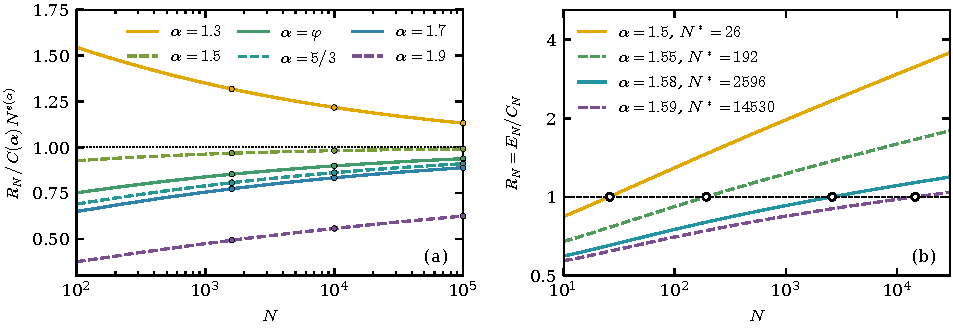
\includegraphics{figures/heavy}
\caption{Alternating runs with a stationary start. (a)
$R_N/(C(\alpha)N^{e(\alpha)})$ for even $N$ from 100 to $10^5$, with the
entries of Table~\ref{tab:heavy} as dots. (b) $R_N$ for
$\alpha=1.5,1.55,1.58,1.59$ below $\varphi$. Each curve crosses 1 once on
$10\le N\le3\cdot10^4$, at $N^*(\alpha)$ (circles).}
\label{fig:heavy}
\end{figure}

\begin{corollary}[the golden-ratio exponent]\label{cor:golden}
Let $1<\alpha<2$ and $e(\alpha)=1-\alpha+1/\alpha$. If
$\Prob(D\ge N)\sim c_DN^{-\beta_D}$ with $c_D,\beta_D>0$, then
$R_N\sim c_DN^{1/\alpha-\beta_D}/(4I_\alpha(2\mu)^{1/\alpha})$. In particular
$R_N\sim C(\alpha)N^{e(\alpha)}$ for the stationary start and
$R_N\sim C_{\rm fr}(\alpha)N^{e(\alpha)-1}$ for the fresh start, where
\[
 C(\alpha)=\frac{\pi\bigl(K_\alpha\lvert\cos\frac{\pi\alpha}2\rvert
 \bigr)^{1/\alpha}}{4(\alpha-1)\Gamma(1+\frac1\alpha)\,
 \zeta(\alpha)^{1+1/\alpha}},\qquad
 C_{\rm fr}(\alpha)=(\alpha-1)\zeta(\alpha)\,C(\alpha).
\]
Since $e(\alpha)>0$ exactly when $\alpha<\varphi$, with a stationary start the
ends win for all large $N$ if $\alpha<\varphi$, and the center wins if
$\alpha>\varphi$. At $\alpha=\varphi$,
\[
 R_N\to C(\varphi)=\frac{\pi\varphi\bigl(\varphi\,\Gamma(\varphi^{-2})\lvert
 \cos\frac{\pi\varphi}2\rvert\bigr)^{1/\varphi}}{4\,\Gamma(\varphi)\,
 \zeta(\varphi)^{\varphi}}=0.7761317206\ldots,
\]
so the center still wins, by the factor $1/C(\varphi)=1.2884\ldots$ in the
limit. That $C(\varphi)<1$ needs no computation (see the proof). With a fresh
start $e(\alpha)-1<0$, and the center wins for every $1<\alpha<2$.
\end{corollary}

\begin{proof}
By Proposition~\ref{prop:edge} and Theorem~\ref{thm:center}, with $h=N/2$, we
have $R_N=\Prob(D\ge N)/(2C_N)$, and this is asymptotic to
$c_DN^{-\beta_D}/(4I_\alpha(2\mu/N)^{1/\alpha})$, which is the general formula.
By Lemma~\ref{lem:stable}(iv),
$4I_\alpha(2\mu)^{1/\alpha}=4\Gamma(1+\frac1\alpha)\mu^{1/\alpha}/(\pi(K_\alpha\lvert\cos\frac{\pi\alpha}2\rvert)^{1/\alpha})$.
The fresh start has $c_D=1$ and $\beta_D=\alpha$, which gives
$C_{\rm fr}(\alpha)$. By Proposition~\ref{prop:edge} the stationary start has
$c_D=1/((\alpha-1)\mu)$ and $\beta_D=\alpha-1$, which gives $C(\alpha)$. Next,
$e(\alpha)=-(\alpha^2-\alpha-1)/\alpha$, and $\varphi$ is the positive root of
$\alpha^2-\alpha-1$. At $\alpha=\varphi$ we have $\alpha-1=1/\varphi$,
$1+1/\alpha=\varphi$ and $2-\alpha=\varphi^{-2}$. So
$K_\varphi=\varphi\,\Gamma(\varphi^{-2})$, and substituting these into
$C(\alpha)$ gives the closed form. To see that $C(\varphi)<1$, use four
elementary bounds. Since $x^{-\varphi}$ is convex, the trapezoid rule
overestimates its integral over $[1,\infty)$, so
$\zeta(\varphi)-\frac12\ge1/(\varphi-1)=\varphi$. The minimum of $\Gamma$ on
$(0,\infty)$ is $0.8856\ldots$~\cite[Section~5.4(iii)]{dlmf}, so
$\Gamma(\varphi)\ge0.8856$. Since $\Gamma\le1$ on $[1,2]$,
$\Gamma(\varphi^{-2})=\Gamma(1+\varphi^{-2})\varphi^2\le\varphi^2$. Finally
$\frac\pi2<\frac{\pi\varphi}2<\frac{5\pi}6$, so
$\lvert\cos\frac{\pi\varphi}2\rvert\le\frac{\sqrt3}2$. Together these give
$C(\varphi)\le\pi\varphi(\sqrt3\varphi^3/2)^{1/\varphi}/(4\cdot0.8856\,(\varphi+\frac12)^\varphi)=0.95136\ldots<1$.
\end{proof}

Corollary~\ref{cor:golden} is the lattice form, with its constant, of the
heuristic of~\cite[Section~6.2.1]{wlh2016}. The approach to $C(\varphi)$ is
slow. At $\alpha=\varphi$ we have $R_{10^5}/C(\varphi)=0.938$, and $R_N$
increases on the computed grid (Table~\ref{tab:heavy} and
Figure~\ref{fig:heavy}).

The golden ratio also appears for the elephant random walk with first step
$+1$ and reversal probability $\varepsilon$. There the law of $A_N$ is
log-concave for every $N$ exactly when
$1-2\varepsilon\le1/\varphi$~\cite[Proposition~2.2]{glrs2025}, and for
$1-2\varepsilon>0.80399$ it is not log-concave for arbitrarily large
$N$~\cite[Theorem~4.4]{tv2026}. We know of no connection.

\begin{remark}[broadened side peaks]\label{rem:humps}
The end bins correspond to the ballistic side peaks of the standard L\'evy
walk, in which every flight has the same speed. These peaks are
$\delta$-functions whose weight decays like $t^{1-\gamma}$ for the
equilibrated start, with $\gamma$ in the role of $\alpha$, while the central
peak has height of order $t^{-1/\gamma}$~\cite[Section~6.2.1]{wlh2016}. With
velocity fluctuations the side peaks broaden into humps. If the speed is
redrawn at each collision, the humps have width of order $t$ and height of
order $t^{-\gamma}$, and if it fluctuates during each flight, they have width
of order $t^{1/2}$ and height of order
$t^{1/2-\gamma}$~\cite[Table~I]{dzh2012}. Matching these heights with
$t^{-1/\gamma}$ gives $\gamma=1$ in the first case, so the center wins for
every $1<\gamma<2$, and in the second case the root
$\gamma=(1+\sqrt{17})/4=1.28\ldots$ of $\gamma^2-\gamma/2-1=0$. So the golden
ratio belongs to the unbroadened peaks, which our lattice walk has.
\end{remark}

\begin{remark}[crossover sizes and heat conduction]\label{rem:crossover}
For $\alpha<\varphi$ and a stationary start the crossover is late when
$\alpha$ is close to $\varphi$. In our computation, for each
$\alpha\in\{1.5,1.55,1.58,1.59\}$, the sign of $R_N-1$ changes exactly once as
$N$ runs over the even numbers in $[10,3\cdot10^4]$, namely at
$N^*(\alpha)=26,192,2596,14530$. Heuristically, $C(\alpha)N^{e(\alpha)}=1$
gives $\log N^*(\alpha)=0.1834/(\varphi-\alpha)+O(1)$ as
$\alpha\uparrow\varphi$. The $O(1)$ term is not small. At $\alpha=1.59$ the
leading term gives $\log N^*\approx6.5$, while the computed value is
$\log14530\approx9.6$. At the value $\alpha=5/3$ of L\'evy-walk models of
heat conduction~\cite{cdp2005,dsd2013,zdk2015}, $R_N\sim C(5/3)N^{-1/15}$ with
$C(5/3)=0.8351$.
\end{remark}

We turn to the other exponents. Table~\ref{tab:outcomes} collects them. For
$\alpha\ge2$ the sums $\tau_m$ have a Gaussian limit, and the center wins
with either start.

\begin{table}[t]
\centering\footnotesize
\setlength{\tabcolsep}{4pt}
\begin{tabular}{@{}lllll@{}}
\toprule
$\alpha$ & start & center $C_N$ & ratio $R_N$ & status\\
\midrule
$\alpha>2$ & stationary & $\sim\sqrt{2\mu/(\pi vN)}$ & $\sim C_2(\alpha)N^{3/2-\alpha}\to0$ & Theorem~\ref{thm:alpha2}(a)\\
$\alpha=2$ & stationary & $\sim\sqrt{2\mu/(\pi N\log N)}$ & $\sim\sqrt{\pi\log N/(8\zeta(2)^3N)}\to0$ & Theorem~\ref{thm:alpha2}(b)\\
$1<\alpha<2$ & stationary & $\sim2I_\alpha(\mu/h)^{1/\alpha}$ & $\sim C(\alpha)N^{e(\alpha)}$ & Corollary~\ref{cor:golden}\\
$1<\alpha<2$ & fresh & $\sim2I_\alpha(\mu/h)^{1/\alpha}$ & $\sim C_{\rm fr}(\alpha)N^{e(\alpha)-1}\to0$ & Corollary~\ref{cor:golden}\\
$\alpha=1$ & fresh & $\approx2/(\pi^2\tilde m_h)$ & $\approx\pi^2\tilde m_h/(8h)\sim\pi^2/(8\log N)$ & heuristic, not proved (Remark~\ref{rem:other})\\
$0<\alpha<1$ & fresh & $\sim\frac2\pi\tan\frac{\pi\alpha}2\cdot\frac1N$ & $\sim\frac{\pi}{4\tan(\pi\alpha/2)}\,N^{1-\alpha}\to\infty$ & Theorem~\ref{thm:lamperti}\\
\bottomrule
\end{tabular}
\caption{The center and the ratio $R_N=E_N/C_N$ for each exponent. The center
wins when $R_N\to0$ and the ends win when $R_N\to\infty$. For $\alpha\ge2$ the
center formula holds for every a.s.\ finite first run, and a fresh start also
gives $R_N\to0$.}
\label{tab:outcomes}
\end{table}

\begin{theorem}[$\alpha\ge2$]\label{thm:alpha2}
Let $D$ be any a.s.\ finite first run, and let $N\to\infty$ over even $N$.
\begin{enumerate}[(a)]
\item Let $\alpha>2$ and
$v=\Var\xi=2\zeta(\alpha-1)-\zeta(\alpha)-\zeta(\alpha)^2$. Then
$C_N\sim\sqrt{2\mu/(\pi vN)}$. With the stationary start
$R_N\sim C_2(\alpha)N^{3/2-\alpha}$, where
$C_2(\alpha)=\sqrt{\pi v/(2\mu)}\big/(2(\alpha-1)\mu)$.
\item Let $\alpha=2$, so that $\mu=\zeta(2)$ and $\E\xi^2=\infty$. Then
$(\tau_m-m\mu)/\sqrt{m\log m}$ converges in law to the standard normal law,
and $C_N\sim\sqrt{2\mu/(\pi N\log N)}$. With the stationary start
$R_N\sim\sqrt{\pi\log N/(8\zeta(2)^3N)}$.
\end{enumerate}
In both cases $R_N\to0$ with the fresh start too.
\end{theorem}

In words, for $\alpha\ge2$ the center is of the Gaussian order $N^{-1/2}$,
with an extra factor $(\log N)^{-1/2}$ at $\alpha=2$, where the variance is
infinite. With either start the end is at most of order $N^{1-\alpha}$, so
the center wins. The
exponent of $R_N$ is continuous at $\alpha=2$, since
$e(2)=-\frac12=\frac32-2$.

\paragraph{Idea of the proof.}
The proof of Theorem~\ref{thm:center} uses the exponent $\alpha$ in three
places only. These are the limit law of $\tau_m$ with its local form, the
bound $u_m(k)\le C_Bmk^{-\alpha-1}$ for a sum far above its mean, and the
fact that the norming sequence varies regularly with index less than $1$. All
three hold for $\alpha\ge2$ with the normal law in place of the stable law.
For $\alpha>2$ the norming is $a_m=\sqrt{vm}$. For $\alpha=2$ the truncated
second moment $\E[\xi^2;\xi\le x]$ grows like $2\log x$, which gives the
norming $a_m=\sqrt{m\log m}$. Since $\int g^2=1/(2\sqrt\pi)$ for the standard
normal density $g$, the center is $1/(\sqrt\pi\,b_h)$ to leading order, where
$b_h$ is the norming at $m=h/\mu$. We give the proof in
Appendix~\ref{app:heavy}, where the proof of Theorem~\ref{thm:center} is
written so that it covers both theorems.

The convergence is slow at $\alpha=2$. There $R_N$ divided by the leading
term in (b) is $0.885$ at $N=1600$ and $0.943$ at $N=10^5$. At $\alpha=3$
the ratio of $R_N$ to the leading term in (a) is $0.981$ at $N=16000$.

For $0<\alpha<1$ the runs have infinite mean, and only the fresh start makes
sense. Then $A_N/N$ has a limit law that is not concentrated at a point,
namely Lamperti's occupation-time
law~\cite{lamperti1958,godrecheluck2001}, with density
\[
 \ell_\alpha(y)=\frac{\sin\pi\alpha}{\pi}\,
 \frac{y^{\alpha-1}(1-y)^{\alpha-1}}{y^{2\alpha}+2y^\alpha(1-y)^\alpha
 \cos\pi\alpha+(1-y)^{2\alpha}}\qquad(0<y<1).
\]
So the center should be of order $1/N$. The next theorem is the local form
of this at the center.

\begin{theorem}[$0<\alpha<1$]\label{thm:lamperti}
Let $0<\alpha<1$, with a fresh start. As $N\to\infty$ over even $N$,
\[
 NC_N\to\ell_\alpha(\tfrac12)=\frac2\pi\tan\frac{\pi\alpha}2 .
\]
Hence $R_N\sim\frac{\pi}{4\tan(\pi\alpha/2)}N^{1-\alpha}\to\infty$.
\end{theorem}

In words, for $\alpha<1$ the center is an ordinary bin of size about $1/N$,
while the end has the much larger probability $\frac12N^{-\alpha}$ that the
first run goes right and lasts all $N$ steps. So the ends win for every $\alpha<1$.
For the continuum L\'evy walk with $0<\gamma<1$, the ballistic regime,
Froemberg et al.~\cite{fsbz2015} find the asymptotic densities.

\paragraph{Idea of the proof.}
Now $\tau_m$ is of order $a_m=m^{1/\alpha}$ with no centering, and $\tau_m/a_m$
converges to a positive stable variable $G$ with density $g$. The number $m$
of runs of each sign is no longer concentrated. It ranges over all $m$ with
$m^{1/\alpha}$ of order $h$, and on this range the terms of
Proposition~\ref{prop:tworenewal} are $\frac2{\alpha hm}t^2g(t)^2$ with
$t=h/a_m$. Summing over $m$ is integrating in $\log m$, which gives
$NC_N\to4\int_0^\infty tg(t)^2\,dt$. This integral is the density at
$\frac12$ of $G_1/(G_1+G_2)$ for two independent copies of $G$, and a Mellin
transform identifies the law of $G_1/G_2$ and hence this density. The proof
is in Appendix~\ref{app:heavy}. It does not use Lamperti's theorem.

Here too the convergence is slow near $\alpha=1$. At $N=16000$ the ratio of
$NC_N$ to its limit is $1.042$, $1.001$, $0.928$ and $0.554$ for
$\alpha=0.3$, $0.5$, $0.7$ and $0.9$. We do not prove the local limit at
bins other than the center.

\begin{remark}[the exponent $\alpha=1$ and the fresh start]\label{rem:other}
With a fresh start the threshold is $\alpha=1$. The ends win for $\alpha<1$
by Theorem~\ref{thm:lamperti}, and the center wins for $\alpha>1$ by
Corollary~\ref{cor:golden} and Theorem~\ref{thm:alpha2}. At $\alpha=1$ we
only have a heuristic. Suppose we repeat the proof of
Theorem~\ref{thm:center} with a skewed Cauchy limit, the centering
$m(H_{m+1}-1)$, and the density $1/\pi^2$ at $0$ of the difference of two
copies of the limit. This suggests the row of Table~\ref{tab:outcomes},
namely $R_N\approx\pi^2\tilde m_h/(8h)\sim\pi^2/(8\log N)$, where
$\tilde m_h$ solves $m(H_{m+1}-1)=h$. We have not controlled the error
terms, so the claim that the center wins by a logarithm at $\alpha=1$ is not
proved. The computed $R_N$ divided by $\pi^2\tilde m_h/(8h)$ is $0.796$,
$0.850$ and $0.886$ at $N=1600$, $10^4$ and $10^5$.
\end{remark}

We do not know a rate in Theorem~\ref{thm:center}, whether $R_N$ is monotone
with a single sign change of $R_N-1$, how to make the case $\alpha=1$
rigorous, or the full shape of $P_N$ for heavy-tailed runs.

\subsection{Aging: the law observed from time $t_a$}\label{sec:aging}

So far the walk starts at step $1$. Now let it start fresh at step $1$ and observe
it from step $t_a+1$ on, for an aging time $t_a=t_a(N)\ge0$. Let $A^{(t_a)}_N$ be the
number of plus steps among the steps $t_a+1,\dots,t_a+N$, and let
$P^{(t_a)}_N(k)=\Prob(A^{(t_a)}_N=k)$. In the physics literature this is the aged
occupation time, and the stationary initial run of Section~\ref{sec:prep-stationary}
is its limit as $t_a\to\infty$ with $N$ fixed. Akimoto, Sera, Yamato and
Yano~\cite{asyy2020} proved the aged form of the arcsine law in distribution for
$0<\alpha<1$, and Akimoto~\cite{akimoto2023} computed the moments of the aged
occupation time for $1<\alpha<2$. Here we give the aged law at every point. The result
is that the bulk does not age, while the atom, the boundary layer and the big-jump
zone do, and each aged piece interpolates between the fresh start at $\theta=0$ and
Corollary~\ref{cor:stationary} at $\theta=\infty$, where $\theta=\lim t_a/N$.

The run in progress at step $t_a+1$ is the initial run of the observed walk. Let
$\Sigma$ be its sign and $D$ the number of its steps from step $t_a+1$ on. Given
$(\Sigma,D)$, the later runs are fresh and alternate. So $P^{(t_a)}_N$ is the law
$P_N$ of Section~\ref{sec:prep-statements} with the initial run
\begin{equation}\label{eq:aged-nu}
 \nu^{(t_a)}_\plus(d)=\sum_{t=0}^{t_a}a_t\,f_\plus(t_a-t+d),\qquad
 \nu^{(t_a)}_\minus(d)=\sum_{t=0}^{t_a}b_t\,f_\minus(t_a-t+d),
\end{equation}
where $a_t$ and $b_t$ are the probabilities that a plus run, respectively a minus
run, starts at step $t+1$ of the fresh walk. Indeed, a plus run that starts at step
$t+1\le t_a+1$ has $d$ steps from step $t_a+1$ on exactly when its length is
$t_a-t+d$. The plus runs start at the renewal epochs of the cycles of the walk,
whose law is $f_\plus*f_\minus$ with mean $s$, so $a_t$ is a renewal sequence and
$b_t=\sum_{t'<t}a_{t'}f_\plus(t-t')$. Under (SPAN) for one sign the support of
$X_\plus+X_\minus$ lies in no progression $b+h\Z$ with $h\ge2$, so by the renewal
theorem~\cite[Section~XIII.3]{feller1968}
\begin{equation}\label{eq:aged-renewal}
 a_t\to\frac1s,\qquad b_t\to\frac1s\qquad(t\to\infty).
\end{equation}
The initial run now depends on $N$ through $t_a$, so the statements of
Theorem~\ref{thm:preparation}, which fix one law, do not apply as stated. Their proofs
do, under one condition on the family. We record this first.

\begin{lemma}[triangular arrays of initial runs]\label{lem:array}
Let the law $\nu^{(N)}$ of the initial run depend on $N$, and suppose that
\begin{equation}\label{eq:tight}
 \varepsilon_J=\sup_N\Prob\bigl(D^{(N)}>J\bigr)\to0\qquad(J\to\infty).
\end{equation}
Then Theorem~\ref{thm:preparation}(a) holds for $P_N$ with the defects computed from
$\nu^{(N)}$. Under the hypotheses of Theorem~\ref{thm:preparation}(c), for every
$\varepsilon>0$ there is $K_0$ such that for $K\ge4K_0$ and all large $N$
\begin{multline}\label{eq:array-decomp}
 \sup_{pN+K\lambda_NB_N\le k\le N}
 \frac{\bigl|P_N(k)-Q^{(N)}_\plus(N)\ones_{\{k=N\}}-G^{\nu^{(N)}}_N(k)-\Psi^{(N)}_N(k)\bigr|}{\widehat G_N(k)}\\
 \le C\Bigl(\varepsilon+r_N+\frac{(1-p)J}{KB_N}+\varepsilon_J\Bigr)
\end{multline}
for every $J\ge1$, with $C$ and $r_N\to0$ depending only on the laws of the runs, and with
$G^{\nu^{(N)}}_N$ and $\Psi^{(N)}_N$ the kernels~\eqref{eq:G-prep} and~\eqref{eq:Psi} of
$\nu^{(N)}$.
\end{lemma}

\begin{proof}
The proof of Theorem~\ref{thm:preparation}(a) in Section~\ref{sec:prep-bulk} uses the law
of the initial run in three places. The weights of $E_1$ have total mass at most $1$,
and the limit~\eqref{eq:prep-shift} does not involve them. The part $E_2$ is at most
$CC_{10}\Prob(D>J)$. The part $E_3$ is the defect, which is kept exactly. So the bound
$\limsup_N\sup_k|e_N(k)|\le(C_1+CC_{10})\Prob(D>J)$ becomes
$(C_1+CC_{10})\varepsilon_J$ for the array, and $J$ is arbitrary. The proof of the
decomposition in (c), Section~\ref{sec:prep-bigjump}, uses the law only through the
total mass of the weights, the tail $\Prob(D>J)$ in Steps 2 and 3, and the kernel
$G^\nu_N$, which records $\pi_\plus$ and $\nu_\minus(d)$ for $d\le j$. Its constants $C$,
$C_*$, $C_{\mathrm G}$, $K_0$, $n_0$ and $r_N$ come from~\eqref{eq:unif-bigjump} and
from (LR) and (RV), so they depend only on the laws of the runs. Step 4 then
gives~\eqref{eq:array-decomp} with $\varepsilon_J$ in place of $\Prob(D>J)$.
\end{proof}

For the aged initial run, $\Prob(D^{(t_a)}>J)=\sum_{t\le t_a}[a_tT_\plus(t_a-t+J+1)+b_tT_\minus(t_a-t+J+1)]
\le\sum_{i>J}(T_\plus(i)+T_\minus(i))$, since $a_t,b_t\le1$, and the right side tends
to zero as $J\to\infty$ because the means are finite. So~\eqref{eq:tight} holds for
every choice of $t_a(N)$. We also need the aged initial run at the scale $N$.

\begin{lemma}[the aged initial run]\label{lem:aged-nu}
Assume (RV) and (SPAN), and let $t_a=t_a(N)\ge0$ be arbitrary.
\begin{enumerate}[(a)]
\item $\nu^{(t_a)}_\sgn(d)\le T_\sgn(d)$ for every $d\ge1$, and
$Q^{(t_a)}_\sgn(N)\le\sum_{i\ge N}T_\sgn(i)$.
\item For every $\varepsilon>0$, uniformly in $d\ge\varepsilon N$,
\[
 \nu^{(t_a)}_\plus(d)=\frac1s\bigl[T_\plus(d)-T_\plus(d+t_a+1)\bigr]+o(T_\plus(N)).
\]
\item If $t_a\to\infty$, then $\nu^{(t_a)}_\sgn(d)\to T_\sgn(d)/s$ for every fixed $d\ge1$,
$\pi^{(t_a)}_\plus=\Prob(\Sigma=\plus)\to p$, and
$Q^{(t_a)}_\plus(N)=(1+o(1))\,s^{-1}\sum_{i=N}^{N+t_a}T_\plus(i)$.
\end{enumerate}
\end{lemma}

\begin{proof}
(a) Since $a_t\le1$, \eqref{eq:aged-nu} gives
$\nu^{(t_a)}_\plus(d)\le\sum_{t\le t_a}f_\plus(t_a-t+d)\le T_\plus(d)$, and summing over
$d\ge N$ gives the bound on the atom.

(b) Write $a_t=1/s+\eta_t$, so $\eta_t\to0$ by~\eqref{eq:aged-renewal}. The main part of
\eqref{eq:aged-nu} is $s^{-1}\sum_{i=d}^{t_a+d}f_\plus(i)=s^{-1}[T_\plus(d)-T_\plus(d+t_a+1)]$.
Fix $M$. The error is at most
$\sup_{t\ge M}|\eta_t|\,T_\plus(d)+M\sup_{i\ge d-M}f_\plus(i)$. Under (RV),
$f_\plus(i)=T_\plus(i)-T_\plus(i+1)=o(T_\plus(i))$, and $T_\plus(i)\le T_\plus(\varepsilon N-M)\le C_\varepsilon T_\plus(N)$
for $i\ge d-M$ and large $N$ by Lemma~\ref{lem:rv}(ii). So the error is at most
$(\sup_{t\ge M}|\eta_t|+o(1))C_\varepsilon T_\plus(N)$, and $M$ is arbitrary.

(c) In~\eqref{eq:aged-nu} put $m=t_a-t$. Then
$\nu^{(t_a)}_\plus(d)=\sum_{m=0}^{t_a}a_{t_a-m}f_\plus(m+d)$, the coefficients are at most $1$,
each tends to $1/s$, and $\sum_mf_\plus(m+d)=T_\plus(d)<\infty$. Dominated convergence
gives $T_\plus(d)/s$, and the minus sign is the same with $b_t$. In the same way
$\pi^{(t_a)}_\plus=\sum_{m=0}^{t_a}a_{t_a-m}T_\plus(m+1)\to s^{-1}\sum_{m\ge0}T_\plus(m+1)=\mu_\plus/s=p$.
For the atom,
$Q^{(t_a)}_\plus(N)=\sum_{i=N}^{N+t_a}a_{t_a+N-i}T_\plus(i)$. Put $\Sigma_N=\sum_{i=N}^{N+t_a}T_\plus(i)$.
Since $T_\plus$ is nonincreasing, Lemma~\ref{lem:rv}(ii) gives
$\Sigma_N\ge\min(t_a,N)\,T_\plus(2N)\ge c\min(t_a,N)\,T_\plus(N)$. Let $M\to\infty$ with
$M=o(\min(t_a,N))$. The $M$ terms with $t_a+N-i<M$ contribute at most $MT_\plus(N)=o(\Sigma_N)$,
and in the other terms the coefficient is $1/s+o(1)$ by~\eqref{eq:aged-renewal}. Hence
$Q^{(t_a)}_\plus(N)=(1/s+o(1))\Sigma_N$.
\end{proof}

By Lemma~\ref{lem:rv}(i) and~(iv), as $N\to\infty$ with $t_a/N\to\theta$,
\begin{equation}\label{eq:aged-sums}
 \sum_{i=N}^{N+t_a}T_\plus(i)\sim
 \begin{cases}
  t_aT_\plus(N)&\text{if }\theta=0\text{ and }t_a\to\infty,\\[2pt]
  NT_\plus(N)\dfrac{1-(1+\theta)^{1-\alpha_\plus}}{\alpha_\plus-1}&\text{if }0<\theta<\infty,\\[6pt]
  NT_\plus(N)\dfrac1{\alpha_\plus-1}&\text{if }\theta=\infty,
 \end{cases}
\end{equation}
and $T_\plus(N+t_a)/T_\plus(N)\to(1+\theta)^{-\alpha_\plus}$, with $(1+\theta)^{-\alpha_\plus}$ read as
$0$ at $\theta=\infty$.

\begin{introtheorem}[aging]\label{thm:aging}
Let the walk start fresh with either sign at step $1$, and let $t_a=t_a(N)\ge0$.
\begin{enumerate}[(a)]
\item (The bulk does not age.) Assume (RV) and (SPAN). For every choice of $t_a(N)$,
\[
 \sup_{1\le k<N}\bigl|B_NP^{(t_a)}_N(k)-h_N(x_{N,k})\bigr|\to0 .
\]
\item (The atom.) Assume (RV) and (SPAN), and let $t_a\to\infty$ with $t_a/N\to\theta\in[0,\infty]$.
Then $P^{(t_a)}_N(N)=Q^{(t_a)}_\plus(N)\sim s^{-1}\sum_{i=N}^{N+t_a}T_\plus(i)$, which
\eqref{eq:aged-sums} evaluates. For $0<\theta<\infty$,
\[
 P^{(t_a)}_N(N)\sim\frac{NT_\plus(N)}{s(\alpha_\plus-1)}\bigl(1-(1+\theta)^{1-\alpha_\plus}\bigr).
\]
\item (The boundary layer.) Assume (RV) and (SPAN), and let $t_a\to\infty$ with
$t_a/N\to\theta\in[0,\infty]$. For every fixed $j\ge1$,
\[
 \frac{P^{(t_a)}_N(N-j)}{T_\plus(N)}\to\kappa^{(\theta)}_\plus(j)
 =p\,u_\minus(j)+\frac1s+\frac1s\bigl(1-(1+\theta)^{-\alpha_\plus}\bigr)\bigl(1+\mu_\plus u_\minus(j)\bigr).
\]
\item (The interior of the big-jump zone.) Assume (RV) and (SPAN) for both signs and (LR)
for the plus sign. For every $\varepsilon\in(0,\frac12)$ and every choice of $t_a(N)$,
uniformly over $k$ with $\varepsilon N\le L_k\le(1-\varepsilon)N$,
\[
 P^{(t_a)}_N(k)=\frac{N-L_k}{\mu_\minus}\,f_\plus(\lfloor L_k\rfloor)
 +\frac{2T_\plus(\lfloor L_k\rfloor)-T_\plus(\lfloor L_k\rfloor+t_a)}{\mu_\minus}+o\bigl(T_\plus(N)\bigr).
\]
If $t_a/N\to\theta\in[0,\infty]$, then for fixed $v\in(p,1)$, with $\ell=(v-p)/(1-p)$,
\[
 \frac{P^{(t_a)}_N(\lfloor vN\rfloor)}{T_\plus(N)}\to I_\plus(v)+\frac{\ell^{-\alpha_\plus}-(\ell+\theta)^{-\alpha_\plus}}{\mu_\minus},
\]
with $I_\plus$ as in Corollary~\ref{cor:infinite-density} and $(\ell+\theta)^{-\alpha_\plus}=0$ at $\theta=\infty$.
\end{enumerate}
The same holds at the minus end with the signs exchanged.
\end{introtheorem}

At $\theta=0$ the atom, the layer and the interior kernel are those of the stationary
initial run with its complete initial run removed, that is $\kappa^{(0)}_\plus=pu_\minus+1/s$
and the kernel of Theorem~\ref{thm:bigjump}(b), while the atom $t_aT_\plus(N)/s$ grows with
$t_a$. At $\theta=\infty$ all four parts are those of Corollary~\ref{cor:stationary}. For
$0<\theta<\infty$ the straddling run reaches the horizon with the probability
$\nu^{(t_a)}_\plus(L_k)\approx s^{-1}[T_\plus(L_k)-T_\plus(L_k+t_a)]$, and this is the term that
ages. The bulk never does.

\begin{proof}
Throughout, $\nu=\nu^{(t_a)}$ is the initial run~\eqref{eq:aged-nu}, which
satisfies~\eqref{eq:tight} by the remark before Lemma~\ref{lem:aged-nu}.

(a) By Lemma~\ref{lem:array}, Theorem~\ref{thm:preparation}(a) holds for $\nu$, and the
proof of part (b) of that theorem shows that the error over $1\le k<N$ is
$\max(\Delta_{\plus,N},\Delta_{\minus,N})+o(1)$. By~\eqref{eq:defect-upper} and
Lemma~\ref{lem:aged-nu}(a),
$\Delta_{\plus,N}\le(1+\mu_\plus)B_N\sup_{d>N/2}\nu_\plus(d)\le(1+\mu_\plus)B_NT_\plus(N/2)$, which
tends to zero by Lemma~\ref{lem:rv}(ii) and~(v). The minus sign is the same.

(b) This is Lemma~\ref{lem:aged-nu}(c) and~\eqref{eq:aged-sums}, together with
$P_N(N)=Q_\plus(N)$ from Proposition~\ref{prop:first-run}.

(c) Fix $j\ge1$ and let $N>2j$. Proposition~\ref{prop:first-run} at $k=N-j$ gives
\[
 P_N(N-j)=\sum_{d=1}^{j}\nu_\minus(d)\,F^\plus_{N-d}(N-j)
 +\sum_{d\le N/2}\nu_\plus(d)\,\Pi^\minus_{N-d}(j)+\sum_{1\le m<N/2}\nu_\plus(N-m)\,\Pi^\minus_m(j),
\]
since $F^\minus_{N-d}(N-j-d)=\Pi^\minus_{N-d}(j)$ and the terms with a minus initial run of
length $d>j$ vanish. We treat the three sums in turn, and we use
$T_\plus(N-d)/T_\plus(N)\to1$ for fixed $d$ and $T_\plus(N-d)\le CT_\plus(N)$ for $d\le N/2$.

For $d\le j$, Theorem~\ref{thm:bigjump}(a) at the horizon $N-d$ and~\eqref{eq:kappa} give
$F^\plus_{N-d}(N-j)/T_\plus(N)\to u_\minus(j-d)$, and $\nu_\minus(d)\to T_\minus(d)/s$ by
Lemma~\ref{lem:aged-nu}(c). The covering identity~\eqref{eq:cover} gives the limit
$s^{-1}\sum_{d=1}^jT_\minus(d)u_\minus(j-d)=1/s$.

In the second sum split at a fixed $J$. For $d\le J$, Theorem~\ref{thm:bigjump}(a) for a
fresh minus start gives $\Pi^\minus_{N-d}(j)/T_\plus(N)\to u_\minus(j)$, and
$\sum_{d\le J}\nu_\plus(d)\to s^{-1}\sum_{d\le J}T_\plus(d)$. For $J<d\le N/2$ the horizon is
at least $N/2$, so $\Pi^\minus_{N-d}(j)\le C_jT_\plus(N)$ for large $N$, and the weights add up
to at most $\varepsilon_J$. Letting $N\to\infty$ and then $J\to\infty$ gives the limit
$pu_\minus(j)$, since $s^{-1}\sum_{d\ge1}T_\plus(d)=p$.

In the third sum, for each fixed $m$, Lemma~\ref{lem:aged-nu}(b) with $d=N-m\ge N/2$
and~\eqref{eq:aged-sums} give
$\nu_\plus(N-m)/T_\plus(N)\to s^{-1}(1-(1+\theta)^{-\alpha_\plus})$. Also
$\nu_\plus(N-m)\le T_\plus(N/2)\le CT_\plus(N)$ for all $m<N/2$ by Lemma~\ref{lem:aged-nu}(a), and
$\sum_{m\ge1}\Pi^\minus_m(j)=1+\mu_\plus u_\minus(j)<\infty$ by Lemma~\ref{lem:green}. Dominated
convergence in $m$ gives the limit $s^{-1}(1-(1+\theta)^{-\alpha_\plus})(1+\mu_\plus u_\minus(j))$.
Adding the three limits gives $\kappa^{(\theta)}_\plus(j)$.

(d) Fix $\varepsilon\in(0,\frac12)$ and let $Z^\varepsilon_N=\{k:\varepsilon N\le L_k\le(1-\varepsilon)N\}$.
On $Z^\varepsilon_N$ we have $j=N-k=(1-p)(N-L_k)\ge(1-p)\varepsilon N$, and
$T_\plus(N)\le\widehat G_N(k)\le C_\varepsilon T_\plus(N)$, as in the proof of
Theorem~\ref{thm:preparation}(e). Since $\lambda_NB_N=o(N)$, the set $Z^\varepsilon_N$ lies in
the zone of~\eqref{eq:array-decomp} for every $K$ once $N$ is large, and it contains no
$k=N$. Letting $N\to\infty$ in~\eqref{eq:array-decomp} with $K=4K_0$, so that
$J/(KB_N)\to0$, then $J\to\infty$, and using that $\varepsilon$ there is arbitrary, we get
\begin{equation}\label{eq:aged-decomp}
 P_N(k)=G^\nu_N(k)+\Psi_N(k)+o\bigl(T_\plus(N)\bigr)\qquad\text{uniformly on }Z^\varepsilon_N .
\end{equation}

\emph{The kernel $G^\nu_N$.} By~\eqref{eq:kappa-prep}, its boundary coefficient is
$\kappa_\plus(j)=\pi_\plus u_\minus(j)+\sum_{d\le j}\nu_\minus(d)u_\minus(j-d)$, and we claim
that $\kappa_\plus(j)\to1/\mu_\minus$ as $j\to\infty$, uniformly in $t_a$. Fix $J$ and split
the sum at $J$. The part $d>J$ is at most $\varepsilon_J$. In the part $d\le J$ each
$u_\minus(j-d)$ tends to $1/\mu_\minus$ as $j\to\infty$ by~\eqref{eq:renewal-thm}, so this part
is $\mu_\minus^{-1}\sum_{d\le J}\nu_\minus(d)+o(1)$, and
$\sum_{d\le J}\nu_\minus(d)=\pi_\minus-\Prob(\Sigma=\minus,D>J)$ differs from $\pi_\minus$ by at
most $\varepsilon_J$. Hence
$|\kappa_\plus(j)-\pi_\plus u_\minus(j)-\pi_\minus/\mu_\minus|\le2\varepsilon_J+o(1)$, and
since $\pi_\plus+\pi_\minus=1$ and $u_\minus(j)\to1/\mu_\minus$ the claim follows. On
$Z^\varepsilon_N$ we have $j\to\infty$ uniformly and $T_\plus(\lfloor L_k\rfloor)\le C_\varepsilon T_\plus(N)$, so
\begin{equation}\label{eq:aged-G}
 G^\nu_N(k)=\frac{N-L_k}{\mu_\minus}f_\plus(\lfloor L_k\rfloor)+\frac{T_\plus(\lfloor L_k\rfloor)}{\mu_\minus}+o\bigl(T_\plus(N)\bigr)
 \qquad\text{uniformly on }Z^\varepsilon_N .
\end{equation}

\emph{The term $\Psi_N$.} Fix $\varepsilon'>0$ and take $R$ and $N_0$ from
Lemma~\ref{lem:green-conc}. Let $k\in Z^\varepsilon_N$, $j=N-k$ and
$\mathcal V=\{d:|d-L_k|\le RB_N\}$. For large $N$ every $d\in\mathcal V$ satisfies
$L_k/2\le d<N$, since $RB_N=o(N)$, so $\mathcal V$ lies in the range of the sum~\eqref{eq:Psi}.
With $m=N-d$ we have $|m-j/(1-p)|=|d-L_k|$, so Lemma~\ref{lem:green-conc} gives
$\sum_{d\notin\mathcal V}\Pi^\minus_{N-d}(j)\le\varepsilon'$, and Lemma~\ref{lem:green} gives
$\sum_{d\in\mathcal V}\Pi^\minus_{N-d}(j)\in[1+\mu_\plus u_\minus(j)-\varepsilon',\,1+\mu_\plus u_\minus(j)]$.
By Lemma~\ref{lem:aged-nu}(a) and Lemma~\ref{lem:rv}(ii), $\nu_\plus(d)\le T_\plus(L_k/2)\le C_\varepsilon T_\plus(N)$
for all $d\ge L_k/2$. By Lemma~\ref{lem:aged-nu}(b), uniformly in $d\in\mathcal V$,
\[
 \nu_\plus(d)-\nu_\plus(\lfloor L_k\rfloor)
 =\frac1s\bigl[T_\plus(d)-T_\plus(\lfloor L_k\rfloor)\bigr]-\frac1s\bigl[T_\plus(d+t_a+1)-T_\plus(\lfloor L_k\rfloor+t_a+1)\bigr]+o(T_\plus(N)),
\]
and both brackets are $o(T_\plus(N))$, because their arguments are at least $\varepsilon N/2$,
differ by at most $RB_N+1=o(N)$, and $T_\plus$ is regularly varying (Lemma~\ref{lem:rv}(i)),
with $T_\plus(\varepsilon N/2)\le C_\varepsilon T_\plus(N)$. Hence
\begin{align*}
 \Bigl|\Psi_N(k)-\nu_\plus(\lfloor L_k\rfloor)\bigl(1+\mu_\plus u_\minus(j)\bigr)\Bigr|
 &\le\sum_{d\notin\mathcal V}\nu_\plus(d)\Pi^\minus_{N-d}(j)
 +\sum_{d\in\mathcal V}\bigl|\nu_\plus(d)-\nu_\plus(\lfloor L_k\rfloor)\bigr|\Pi^\minus_{N-d}(j)\\
 &\quad+\nu_\plus(\lfloor L_k\rfloor)\,\varepsilon'\\
 &\le C_\varepsilon\varepsilon'T_\plus(N)+(1+\mu_\plus)\,o(T_\plus(N))+C_\varepsilon\varepsilon'T_\plus(N),
\end{align*}
uniformly on $Z^\varepsilon_N$. Since $\varepsilon'$ is arbitrary, and since
$1+\mu_\plus u_\minus(j)\to1+\mu_\plus/\mu_\minus=s/\mu_\minus$ uniformly on $Z^\varepsilon_N$,
Lemma~\ref{lem:aged-nu}(b) gives
\begin{equation}\label{eq:aged-Psi}
 \Psi_N(k)=\frac{s}{\mu_\minus}\,\nu_\plus(\lfloor L_k\rfloor)+o(T_\plus(N))
 =\frac{T_\plus(\lfloor L_k\rfloor)-T_\plus(\lfloor L_k\rfloor+t_a+1)}{\mu_\minus}+o\bigl(T_\plus(N)\bigr).
\end{equation}
Now~\eqref{eq:aged-decomp}, \eqref{eq:aged-G} and~\eqref{eq:aged-Psi} give the expansion, since
$T_\plus(\lfloor L_k\rfloor+t_a)-T_\plus(\lfloor L_k\rfloor+t_a+1)=f_\plus(\lfloor L_k\rfloor+t_a)\le\sup_{i\ge\varepsilon N}f_\plus(i)=o(T_\plus(N))$.
For $k=\lfloor vN\rfloor$ with $v\in(p,1)$ fixed we have $L_k=\ell N+O(1)$, and as in the proof
of Corollary~\ref{cor:infinite-density}, (LR) and (RV) give
$(N-L_k)f_\plus(\lfloor L_k\rfloor)/T_\plus(N)\to\alpha_\plus(1-\ell)\ell^{-\alpha_\plus-1}$ and
$T_\plus(\lfloor L_k\rfloor)/T_\plus(N)\to\ell^{-\alpha_\plus}$, while
$T_\plus(\lfloor L_k\rfloor+t_a)/T_\plus(N)\to(\ell+\theta)^{-\alpha_\plus}$ when $t_a/N\to\theta$. The
minus end is the mirror image.
\end{proof}

The golden ratio threshold of Theorem~\ref{thm:mode}(d) survives aging. In its proof,
parts (a) and (b) of Theorem~\ref{thm:mode} use the initial run only
through~\eqref{eq:mode-interior}, which is Theorem~\ref{thm:aging}(a) for the aged law.

\begin{corollary}[the golden ratio under aging]\label{cor:aged-mode}
Assume (RV) and (SPAN), a fresh start at step $1$ and $t_a/N\to\theta\in(0,\infty]$. The
endpoint of sign $\sgn$ beats every interior value of $P^{(t_a)}_N$ for all large $N$ when
$\alpha_\sgn-1<1/\alpha_*$, and loses to the largest interior value when
$\alpha_\sgn-1>1/\alpha_*$. With equal indices $\alpha_\plus=\alpha_\minus=\alpha$ the global mode
is an endpoint for all large $N$ when $\alpha<\varphi$ and is interior for all large $N$ when
$\alpha>\varphi$. For $T_\plus(n)=T_\minus(n)=n^{-\alpha}$ and $0<\theta<\infty$,
$B_NP^{(t_a)}_N(N)/H_N\sim(1-(1+\theta)^{1-\alpha})\,\mathcal C(\alpha)N^{1-\alpha+1/\alpha}$, so at
$\alpha=\varphi$ the mode is interior for every $\theta$.
\end{corollary}

\begin{proof}
By Theorem~\ref{thm:aging}(a), \eqref{eq:mode-interior} holds for the aged law, so parts (a)
and (b) of Theorem~\ref{thm:mode} hold for it with the same proof. By
Theorem~\ref{thm:aging}(b) and~\eqref{eq:aged-sums}, $P^{(t_a)}_N(N)$ is asymptotic to a
constant multiple of $NT_\plus(N)$, which is regularly varying with index $1-\alpha_\plus$, and
$B_N\in\RV_{1/\alpha_*}$ by Lemma~\ref{lem:rv}(v). So $B_NP^{(t_a)}_N(N)/H_N$ tends to infinity or
to zero according to the sign of $1/\alpha_*-(\alpha_\plus-1)$, and part (b) of
Theorem~\ref{thm:mode} concludes. The minus end is the same. With equal indices the
condition $\alpha-1<1/\alpha$ is $\alpha<\varphi$. For the pure power laws the computation in
the proof of Theorem~\ref{thm:mode}(d) applies with the atom multiplied by
$1-(1+\theta)^{1-\alpha}<1$, and $\mathcal C(\varphi)<1$.
\end{proof}

For $t_a=o(N)$ the atom is $t_aT_\plus(N)/s$ by Theorem~\ref{thm:aging}(b), and the comparison
with the bulk depends on the rate at which $t_a$ grows. For the fresh start itself the mode
is interior by Theorem~\ref{thm:mode}(d). Section~\ref{sec:verify} reports a check of parts (b)
and (c) against the exact aged law.

\section{Verification}\label{sec:verify}

{\sloppy
All computations are in Python, and the main ones were done by two independent
methods. No proof in this paper rests on a computation. The tables,
the figures and the numbers quoted outside the proofs rest on computation
alone. The script \texttt{verify\_heavy\_runs.py} recomputes the numbers of
Section~\ref{sec:heavy} and Appendix~\ref{app:heavy}, the script \texttt{verify\_aging.py}
those of Section~\ref{sec:aging} and Appendix~\ref{app:aging}, and
\texttt{verify\_aging\_urn.py} checks Proposition~\ref{prop:aging-urn} in exact arithmetic for
two, three and four states.

Some of the exact and finite statements are also proved in Lean~4, among
them Proposition~\ref{prop:aging-two} and the identities
behind Corollary~\ref{cor:golden}. The Lean files are in the folder
\nolinkurl{kagey-problems/problem131/lean/PaperD}, which this paper shares with Paper~D. The file
\nolinkurl{MAP.md} in that folder lists each formalized statement with its
Lean name. The
asymptotic results and Theorem~\ref{thm:aging-d} were not formalized.

The scripts and the Lean files are in the repository named under ``Data
availability'' at the end of the paper, which also says how to rerun the
checks.
\par}


\paragraph{Acknowledgments.} I thank Peter Kagey for posing the problem and
Aidan Deshong for insightful conversations.

\section*{A note on the use of AI}
% AI NOTE: to be written by the author.
All mathematical claims, proofs and computations in this paper are my
responsibility.

\appendix
\section{Proofs for Section~\ref{sec:heavy}}\label{app:heavy}

We use the notation of Section~\ref{sec:heavy}, with $\tau_0=0$. For a first run $D$ let
$\tau^D_m=D+\tau'_{m-1}$, where $(\tau'_m)$ is an independent copy of $(\tau_m)$, and
$\tau^D_0=0$. Then $u^D_m(k)=\Prob(\tau^D_m=k)$ and
$q^D_m(k)=\Prob(\tau^D_{m-1}<k\le\tau^D_m)$. We find each of these by conditioning on
where the run before ends. For example, the $m$-th run covers level $k$ exactly when the
first $m-1$ runs end at some level $k-j$ with $j\ge1$ and the $m$-th run has length at
least $j$. In this way, for $m,k\ge1$,
\begin{equation}\label{eq:C-conv}
\begin{gathered}
q_m(k)=\sum_{j\ge1}\bar F(j)\,u_{m-1}(k-j),\qquad
q^D_{m+1}(k)=\sum_{j\ge1}\bar F(j)\,u^D_m(k-j),\\
u^D_m(k)=\sum_{\ell\ge1}\Prob(D=\ell)\,u_{m-1}(k-\ell).
\end{gathered}
\end{equation}
Here $u_0(k)=\mathbf 1\{k=0\}$. The sums $\tau_m$ and $\tau^D_m$ increase strictly in $m$.
So exactly one run covers a given level $k\ge1$, and at most one run ends there. Hence
$\sum_mq_m(k)=\sum_mq^D_m(k)=1$ and $\sum_mu_m(k)\le1$, $\sum_mu^D_m(k)\le1$. Also, the
first $m'$ runs reach level $k$ exactly when one of them covers it, so
$\sum_{m\le m'}q_m(k)=\Prob(\tau_{m'}\ge k)$, and in the same way
$\sum_{m\le m'}q^D_m(k)=\Prob(\tau^D_{m'}\ge k)$.

Sections~\ref{app:heavy-setting} to~\ref{app:heavy-alpha2} treat $\alpha>1$ and prove
Theorems~\ref{thm:center} and~\ref{thm:alpha2} together.
Section~\ref{app:heavy-lamperti} treats $0<\alpha<1$ and proves
Theorem~\ref{thm:lamperti}.

\subsection{The setting for \texorpdfstring{$\alpha>1$}{alpha > 1}}\label{app:heavy-setting}

Let $\alpha>1$, so that $\mu=\zeta(\alpha)<\infty$. The proof of the center asymptotics uses
the exponent only through the following three facts about a norming sequence $(a_m)$ of
positive numbers.
\begin{enumerate}[(F1)]
\item For $m\ge3$ we have $a_m=a(m)$, where $a(x)=c_ax^{\kappa}(\log x)^{\beta}$ on
$[3,\infty)$ with constants $c_a>0$, $0<\kappa<1$ and $\beta\ge0$.
\item The variables $(\tau_m-m\mu)/a_m$ converge in law to a variable $G$ that has a
bounded, uniformly continuous density $g$ with $g(z)\to0$ as $\lvert z\rvert\to\infty$.
With $z_{m,k}=(k-m\mu)/a_m$, the numbers
$\delta_m=\sup_k\lvert a_mu_m(k)-g(z_{m,k})\rvert$ tend to $0$, and
$\bar u=\sup_{m\ge1}\sup_ka_mu_m(k)$ is finite.
\item There is a constant $C_B$ such that $u_m(k)\le C_B\,m\,k^{-\alpha-1}$ for all
$m\ge1$ and $k\ge2m\mu$.
\end{enumerate}
The function $a$ in (F1) is increasing, and $a(\lambda x)/a(x)\to\lambda^\kappa$ as
$x\to\infty$, uniformly for $\lambda$ in a compact subset of $(0,\infty)$. So
$a_m\to\infty$ and $a_m/a_{m-1}\to1$. For $1<\alpha<2$ we take $a_m=m^{1/\alpha}$. Then
(F1) holds with $\kappa=1/\alpha$ and $\beta=0$, (F2) is Lemma~\ref{lem:stable}(ii)
and~(iii), and (F3) is Lemma~\ref{lem:C-bigjump} below. We write $\omega$ for the modulus
of continuity of $g$ and $\bar g(x)=\sup_{\lvert y\rvert\ge x}g(y)$. So
$\omega(\eta)\to0$ as $\eta\to0$ and $\bar g(x)\to0$ as $x\to\infty$.

\subsection{Two lemmas on renewal sums}

A sum of $m$ runs that is much larger than its mean is most likely made by a single long
run. The first lemma turns this into a local bound. Bounds of this kind are
classical in the big-jump domain~\cite{dds2008}. We include a short
proof to keep the paper self-contained.

\begin{lemma}\label{lem:C-bigjump}
Let $\alpha>1$. There is a constant $C_B=C_B(\alpha)$ such that
$u_m(k)\le C_B\,m\,k^{-\alpha-1}$ for all $m\ge1$ and $k\ge2m\mu$.
\end{lemma}

\begin{proof}
We split the event $\{\tau_m=k\}$ according to whether some run is long, namely at least
$y=k/r$, where $r>2$ is a constant that depends only on $\alpha$ and is chosen below. The
first part is small because one run takes a given value $\ell\ge y$ with probability at
most $\alpha y^{-\alpha-1}$. If no run is long, then $\tau_m$ is a sum of variables below $y$ whose mean is at most $k/2$,
and a Chernoff bound shows that such a sum rarely reaches $k$. Here $C$ depends only on
$\alpha$ and may change from line to line. Since $\mu\ge1$ we have $m\le k/2$.

\emph{One big jump.} By the mean value theorem
$\Prob(\xi=\ell)=\ell^{-\alpha}-(\ell+1)^{-\alpha}\le\alpha\ell^{-\alpha-1}$. Fix an
index $i$. Then
\[
\Prob(\tau_m=k,\,\xi_i\ge y)=\sum_{\ell\ge y}\Prob(\xi=\ell)\,\Prob(\tau_m-\xi_i=k-\ell)
\le\alpha y^{-\alpha-1}=\alpha r^{\alpha+1}k^{-\alpha-1},
\]
because the first factor is at most $\alpha y^{-\alpha-1}$ and the second factors add up
to at most $1$. The $m$ indices together give at most $\alpha r^{\alpha+1}mk^{-\alpha-1}$.

\emph{No big jump.} We may take $y\ge1$, since otherwise $\max_i\xi_i<y$ is impossible.
Let $x_0>0$ and $s\ge0$. For $0\le x\le s$ we have
$e^x\le1+x+\frac{x^2}2e^s$. We use this with $x=s\xi/y$ on the event $\{\xi<y\}$ and then
$1+x\le e^x$. This gives
$\E[e^{s\xi/y};\xi<y]\le\exp\bigl(\frac sy\E[\xi;\xi<y]+\frac{s^2e^s}{2y^2}\E[\xi^2;\xi<y]\bigr)$.
By independence and Markov's inequality for $e^{s\tau_m/y}$,
\begin{equation}\label{eq:C-chernoff}
\Prob\bigl(\tau_m\ge x_0,\ \max_{i\le m}\xi_i<y\bigr)
\le\exp\Bigl(-\frac{sx_0}y+m\Bigl(\frac sy\,\E[\xi;\xi<y]
+\frac{s^2e^s}{2y^2}\,\E[\xi^2;\xi<y]\Bigr)\Bigr).
\end{equation}
We take $x_0=k$. Since $\E[\xi;\xi<y]\le\mu$ and $k-m\mu\ge k/2$, the first two terms of
the exponent add up to at most $-\frac sy\cdot\frac k2=-sr/2$. So the exponent is at most
$-sr/2+\frac12r^2s^2e^s\,m\,k^{-2}\,\E[\xi^2;\xi<y]$. It remains to choose $s$ and $r$ so that the bound is at most $Cmk^{-\alpha-1}$. The
choice depends on how fast the truncated second moment grows, so there are three cases.

Let $1<\alpha<2$. Then $\E[\xi^2;\xi<y]\le\alpha\sum_{\ell<y}\ell^{1-\alpha}\le
Cy^{2-\alpha}$, so the exponent is at most $-sr/2+Cr^\alpha s^2e^sm/k^\alpha$. Take
$s=\frac12\log(k^\alpha/m)$, which is positive since $m\le k/2<k^\alpha$. Then
$e^sm/k^\alpha=e^{-s}$ and $s^2e^{-s}\le1$, so the second term is at most $Cr^\alpha$.
The first term is $-\frac r4\log(k^\alpha/m)$. So the probability is at most
$C(m/k^\alpha)^{r/4}$. We take $r=4+4/(\alpha-1)$, so that $r/4=1+1/(\alpha-1)$. Since
$m\le k$, the bound is at most
$C(m/k^\alpha)(k^{1-\alpha})^{1/(\alpha-1)}=Cmk^{-\alpha-1}$.

Let $\alpha>2$. Then $\E[\xi^2;\xi<y]\le\E\xi^2<\infty$, so the exponent is at most
$-sr/2+Cr^2s^2e^sm/k^2$. Take $s=\frac12\log(k^2/m)$, which is positive since $m<k^2$.
As before the probability is at most $C(m/k^2)^{r/4}$. With $r=4\alpha$ and $m\le k$
this is $C\,m\,m^{\alpha-1}k^{-2\alpha}\le Cmk^{-\alpha-1}$.

Let $\alpha=2$. Then $\E[\xi^2;\xi<y]\le2\sum_{\ell<y}\ell^{-1}\le2\log(ek)$, so the
exponent is at most $-sr/2+r^2s^2e^sm\log(ek)/k^2$. Take
$s=\frac12\log\frac{k^2}{m\log(ek)}$, which is positive since
$m\log(ek)\le\frac12k\log(ek)<k^2$. As before the probability is at most
$C(m\log(ek)/k^2)^{r/4}$. With $r=20$ and $m\le k$ this is at most
$Cmk^{-6}\log^5(ek)\le Cmk^{-3}$.

In each case the two bounds together give the lemma.
\end{proof}

\begin{lemma}\label{lem:C-firstpassage}
Let $\alpha>1$ and assume \textup{(F1)} and \textup{(F2)}. Let $D$ be any a.s.\ finite
first run. Then
\[
\sup_k\Bigl\lvert\frac{a_m}\mu q_m(k)-g(z_{m,k})\Bigr\rvert,\qquad
\sup_k\bigl\lvert a_mu^D_m(k)-g(z_{m,k})\bigr\rvert,\qquad
\sup_k\Bigl\lvert\frac{a_m}\mu q^D_{m+1}(k)-g(z_{m,k})\Bigr\rvert
\]
tend to $0$ as $m\to\infty$. For $m\ge2$, $\sup_kq_m(k)\le\mu \bar u/a_{m-1}$ and
$\sup_ku^D_m(k)\le \bar u/a_{m-1}$.
\end{lemma}

\begin{proof}
By \eqref{eq:C-conv}, $q_m$ and $u^D_m$ are sums of shifts of $u_{m-1}$ with total
weights $\sum_j\bar F(j)=\mu$ and $1$. Since $u_{m-1}(k)\le\bar u/a_{m-1}$, this gives the
two bounds for $m\ge2$.

For the limits we use that a shift by a bounded amount $j$ moves the point $z_{m,k}$ only
by $O(1/a_m)$, and that $g$ is uniformly continuous. So the local limit for $u_{m-1}$
passes to these sums. We give the details for $q_m$. Fix $J\ge1$ and $Z>0$, put
$\sigma_J=\sum_{j>J}\bar F(j)$ and write $z=z_{m,k}$. We compare term by term the two sums
\[
a_{m-1}q_m(k)=\sum_{j\ge1}\bar F(j)\,a_{m-1}u_{m-1}(k-j)\qquad\text{and}\qquad
\mu g(z)=\sum_{j\ge1}\bar F(j)\,g(z).
\]
The terms with $j>J$ add up to at most $\bar u\sigma_J$ in the first sum and
$\lVert g\rVert_\infty\sigma_J$ in the second.

Let $j\le J$. By (F2),
$\lvert a_{m-1}u_{m-1}(k-j)-g(z_{m-1,k-j})\rvert\le\delta_{m-1}$. Next we compare
$g(z_{m-1,k-j})$ with $g(z)$. The definition of $z_{m,k}$ gives
$z_{m-1,k-j}=z\,a_m/a_{m-1}+(\mu-j)/a_{m-1}$. If $\lvert z\rvert\le Z$, then
$\lvert z_{m-1,k-j}-z\rvert\le\eta_m$ with
$\eta_m=Z\lvert a_m/a_{m-1}-1\rvert+(J+\mu)/a_{m-1}$, so the two values of $g$ differ by
at most $\omega(\eta_m)$. If $\lvert z\rvert>Z$, then
$\lvert z_{m-1,k-j}\rvert\ge Z/2$ once $m$ is large (how large depends only on $J$ and
$Z$), so both values lie in $[0,\bar g(Z/2)]$. In both cases they differ by at most
$\omega(\eta_m)+\bar g(Z/2)$. Hence, uniformly in $k$ for large $m$,
\[
\bigl\lvert a_{m-1}q_m(k)-\mu g(z)\bigr\rvert
\le\mu\bigl(\delta_{m-1}+\omega(\eta_m)+\bar g(Z/2)\bigr)
+(\bar u+\lVert g\rVert_\infty)\sigma_J .
\]
Here $\eta_m\to0$ as $m\to\infty$. So we let $m\to\infty$ and then $J,Z\to\infty$, and
the right side tends to $0$. Since $a_m/a_{m-1}\to1$ and $a_{m-1}q_m(k)\le\mu\bar u$, we
may replace $a_{m-1}$ by $a_m$ on the left. This gives the first limit.

The second limit follows in the same way from the sum for $u^D_m$, with the weights
$\Prob(D=\ell)$ and with $\Prob(D>J)$ in place of $\sigma_J$, which tends to $0$ as
$J\to\infty$ because $D$ is a.s.\ finite. The third follows from the sum for $q^D_{m+1}$, with
$a_mu^D_m$ in place of $a_{m-1}u_{m-1}$, the second limit in place of $\delta_{m-1}\to0$,
and the shift $z_{m,k-j}-z_{m,k}=-j/a_m$. For the terms with $j>J$ we use the bound
$a_mu^D_m(k)\le\bar u\,a_m/a_{m-1}$ from above in place of $\bar u$, and $a_m/a_{m-1}$ is
bounded since it tends to $1$.
\end{proof}

\subsection{The center for \texorpdfstring{$\alpha>1$}{alpha > 1}}

\begin{proposition}\label{prop:C-center}
Let $\alpha>1$ and assume \textup{(F1)}, \textup{(F2)} and \textup{(F3)}. Let $D$ be any
a.s.\ finite first run and put $b_h=a(h/\mu)$. As $N=2h\to\infty$,
\[
C_N\sim\frac2{b_h}\int_{\mathbb R}g(z)^2\,dz .
\]
\end{proposition}

\paragraph{Idea of the proof.}
We split the sum in Proposition~\ref{prop:tworenewal} by the number $m$ of runs into four
regions. In the main region $\lvert m\mu-h\rvert\le Mb_h$ both factors are given by the
local limit theorem, and the terms form a Riemann sum for $2b_h^{-1}\int_{-M}^Mg^2$. For
$m\le h/(4\mu)$ the level $h$ is far above the mean of $\tau_m$, and (F3) makes these terms
$O(h^{-\alpha})$. In the other two regions (the $m$ between these two, and the $m$ above
the main region) one factor of each term is $O(1/b_h)$, and the other factors add up to a
tail probability of $G$, which is small when $M$ is large.

\begin{proof}
By Proposition~\ref{prop:tworenewal},
$C_N=\sum_{m\ge1}\bigl[u_m(h)q^D_{m+1}(h)+u^D_m(h)q_m(h)\bigr]$. Fix $M>1$, put
$m_\pm=(h\pm Mb_h)/\mu$, and let $\Sigma_1,\dots,\Sigma_4$ be the parts of this sum over
the regions $\mathcal R_1=\{m\le h/(4\mu)\}$, $\mathcal R_2=\{h/(4\mu)<m<m_-\}$,
$\mathcal R_3=\{m_-\le m\le m_+\}$ and $\mathcal R_4=\{m>m_+\}$. We show that
$b_h\Sigma_3$ tends to $2\int_{-M}^Mg^2$ and that the other three parts are small.

We need three consequences of (F1). First, $b_h=o(h)$ and $h^{-\alpha}=o(1/b_h)$, since
$\kappa<1<\alpha$. Second, $a(h/(8\mu))\ge b_h/9$ and $a(h/(2\mu))\ge b_h/3$ for large
$h$, since $8^{-\kappa}>\frac19$ and $2^{-\kappa}>\frac13$. Third, $a_m/b_h\to1$
uniformly in $m$ with $\lvert m\mu-h\rvert\le2Mb_h$.

\emph{Region $\mathcal R_1$ (far too few runs).} Here $h\ge4m\mu$, so level $h$ is far above
the mean of $\tau_m$. We show that $u_m(h)$ and $q_m(h)$ are both $O(h^{-\alpha})$ for
$m\in\mathcal R_1$. By (F3), $u_m(h)\le C_Bmh^{-\alpha-1}\le C_Bh^{-\alpha}/(4\mu)$. Also
$q_1(h)=h^{-\alpha}$. For $m\ge2$ we split the sum for $q_m(h)$ in~\eqref{eq:C-conv} at
$j=h/2$. The terms with $j\ge h/2$ have $\bar F(j)\le(h/2)^{-\alpha}$, and the factors
$u_{m-1}(h-j)$ add up to at most $1$. So these terms add up to at most
$(h/2)^{-\alpha}$. For $j<h/2$ we have $h-j>h/2\ge2\mu(m-1)$, so (F3) applies to
$u_{m-1}(h-j)$, and the weights $\bar F(j)$ add up to at most $\mu$. So the other terms
add up to at most $\mu C_B(m-1)(h/2)^{-\alpha-1}\le2^{\alpha-1}C_Bh^{-\alpha}$. In
$\Sigma_1$ each of these factors is multiplied by $q^D_{m+1}(h)$ or by $u^D_m(h)$, and
$\sum_mq^D_{m+1}(h)\le1$ and $\sum_mu^D_m(h)\le1$. Hence $\Sigma_1=O(h^{-\alpha})$, which
is $o(1/b_h)$.

\emph{Region $\mathcal R_2$ (too few runs).} In each term one
factor is at most $9\bar u/b_h$, and the other factors add up to the probability that few
runs reach level $h$. For large $h$ we have $m-1\ge h/(8\mu)$ here, so
$a_m\ge a_{m-1}\ge b_h/9$ and $u_m(h),u^D_m(h)\le9\bar u/b_h$ by (F2) and
Lemma~\ref{lem:C-firstpassage}. Let $m'=\lfloor m_-\rfloor$. Every $m\in\mathcal R_2$ is
at most $m'$, so $\sum_{m\in\mathcal R_2}q_m(h)\le\Prob(\tau_{m'}\ge h)$ and
$\sum_{m\in\mathcal R_2}q^D_{m+1}(h)\le\Prob(D+\tau'_{m'}\ge h)$. The last probability
is at most $\Prob(D\ge b_h)+\Prob(\tau_{m'}\ge h-b_h)$. Since $m'\mu\le h-Mb_h$ and
$a_{m'}\le b_h$, the event $\{\tau_{m'}\ge h-b_h\}$ implies
$(\tau_{m'}-m'\mu)/a_{m'}\ge M-1$. Now $\Prob(D\ge b_h)\to0$ because $D$ is a.s.\
finite, and $(\tau_{m'}-m'\mu)/a_{m'}$ converges in law to $G$, which has a continuous
law. So $\limsup_hb_h\Sigma_2\le18\bar u\,\Prob(G\ge M-1)$.

\emph{Region $\mathcal R_4$ (too many runs).} This is like $\mathcal R_2$. For large $h$
we have $m-1\ge h/(2\mu)$ here, so $u_m(h),u^D_m(h)\le3\bar u/b_h$. Let
$m''=\lfloor m_+\rfloor$. The runs after the first $m''$ cover level $h$ exactly when
the first $m''$ do not reach it. So $\sum_{m\in\mathcal R_4}q_m(h)=\Prob(\tau_{m''}<h)$
and, since $D\ge1$,
$\sum_{m\in\mathcal R_4}q^D_{m+1}(h)=\Prob(D+\tau'_{m''}<h)\le\Prob(\tau_{m''}<h)$. Now
$m''\mu>h+Mb_h-\mu$, so $(h-m''\mu)/a_{m''}\le(\mu-Mb_h)/a_{m''}\to-M$. Hence
$\limsup_hb_h\Sigma_4\le6\bar u\,\Prob(G\le-M)$.

\emph{Region $\mathcal R_3$ (the main part).} Here $m\to\infty$ and
$a_m=b_h(1+o(1))$ uniformly. By (F2) and Lemma~\ref{lem:C-firstpassage}, the factors
$u_m(h)$ and $u^D_m(h)$ are $(g(z_{m,h})+o(1))/a_m$, and the factors $q_m(h)$ and
$q^D_{m+1}(h)$ are $\mu(g(z_{m,h})+o(1))/a_m$. So, uniformly in $m\in\mathcal R_3$,
\[
u_m(h)q^D_{m+1}(h)+u^D_m(h)q_m(h)=\frac{2\mu}{a_m^2}\bigl(g(z_{m,h})^2+o(1)\bigr).
\]
Put $y_m=(h-m\mu)/b_h$. Then $z_{m,h}=y_mb_h/a_m$ and $\lvert y_m\rvert\le M$, so
$\lvert z_{m,h}-y_m\rvert\le M\lvert b_h/a_m-1\rvert\to0$ and
$g(z_{m,h})^2=g(y_m)^2+o(1)$. The $y_m$ with $m\in\mathcal R_3$ are the points of an
arithmetic progression with step $\mu/b_h$ that lie in $[-M,M]$. There are at most
$2Mb_h/\mu+1$ of them, so the $o(1)$ terms below add up to $o(1)$, and the rest is a
Riemann sum. Hence
\[
b_h\Sigma_3=2\bigl(1+o(1)\bigr)\frac\mu{b_h}
\sum_{m\in\mathcal R_3}\bigl(g(y_m)^2+o(1)\bigr)\to2\int_{-M}^Mg^2 .
\]
Adding the four regions,
\[
\limsup_{h\to\infty}\Bigl\lvert b_hC_N-2\int g^2\Bigr\rvert
\le2\int_{\lvert z\rvert>M}g^2+18\bar u\,\Prob(G\ge M-1)+6\bar u\,\Prob(G\le-M),
\]
and letting $M\to\infty$ gives $C_N\sim2b_h^{-1}\int g^2$.
\end{proof}

\begin{proof}[Proof of Theorem~\ref{thm:center}]
Let $1<\alpha<2$ and $a_m=m^{1/\alpha}$. As noted in
Section~\ref{app:heavy-setting}, (F1) to (F3) hold, with $b_h=(h/\mu)^{1/\alpha}$. So
Proposition~\ref{prop:C-center} gives $C_N\sim2I_\alpha(\mu/h)^{1/\alpha}$, and the
second form follows from Lemma~\ref{lem:stable}(iv) and $h=N/2$.
\end{proof}

\subsection{Proof of Theorem~\ref{thm:alpha2}}\label{app:heavy-alpha2}

We apply Proposition~\ref{prop:C-center} with the standard normal density in place of the
stable density. So let $\alpha\ge2$ and let $g$ be the standard normal density. We have
to find a norming sequence $(a_m)$ with (F1), (F2) and (F3). Fact (F3) is
Lemma~\ref{lem:C-bigjump}, which holds for every $\alpha>1$. For (F2) it is enough that
$(\tau_m-m\mu)/a_m$ converges in law to the standard normal law. Indeed, $g$ is bounded
and uniformly continuous and vanishes at $\pm\infty$. Every $\Prob(\xi=k)$ is positive,
so $\xi$ has maximal span $1$, and Gnedenko's local limit
theorem~\cite[Theorem~4.2.1]{ibragimovlinnik1971} turns the convergence in law into
$\delta_m\to0$. Then $\bar u<\infty$ follows as in the proof of
Lemma~\ref{lem:stable}(iii). So in each of the two cases we choose $(a_m)$, check (F1)
and the normal limit, and read off $b_h=a(h/\mu)$. Since $\int g^2=1/(2\sqrt\pi)$,
Proposition~\ref{prop:C-center} then gives $C_N\sim1/(\sqrt\pi\,b_h)$.

(a) Let $\alpha>2$. Then $\xi$ has a finite variance, and we use the central limit
theorem. Summation by parts gives
$\E\xi^2=\sum_{k\ge1}(2k-1)\bar F(k)=2\zeta(\alpha-1)-\zeta(\alpha)$, so $v=\E\xi^2-\mu^2$
is as stated and finite. It is positive because $\xi$ is not constant. We take
$a_m=\sqrt{vm}$. This has (F1) with $\kappa=\frac12$ and $\beta=0$, and the central limit
theorem gives the normal limit. So $b_h=\sqrt{vh/\mu}$, and with $h=N/2$ we get
$C_N\sim(\pi vh/\mu)^{-1/2}=\sqrt{2\mu/(\pi vN)}$. For the stationary start
Proposition~\ref{prop:edge} gives $E_N=N^{1-\alpha}(1+O(1/N))/(2(\alpha-1)\mu)$.
Dividing $E_N$ by $C_N$ gives $R_N\sim C_2(\alpha)N^{3/2-\alpha}$.

(b) Let $\alpha=2$, so that $\mu=\zeta(2)$ and $\E\xi^2=\infty$. The central limit
theorem with the norming $\sqrt m$ fails, but the variance is infinite only by a
logarithm, and the limit is still normal with a slightly larger norming. To see this we
compute the truncated second moment
\[
U(x)=\E[\xi^2;\xi\le x]=\sum_{k\le x}k^2\bigl(k^{-2}-(k+1)^{-2}\bigr)
=\sum_{k\le x}\frac{2k+1}{(k+1)^2}=2\log x+O(1).
\]
This function varies slowly. So $\xi$ is in the domain of attraction of the normal law,
and $(\tau_m-m\mu)/a_m$ converges in law to the standard normal law for every sequence
$(a_m)$ with
$mU(a_m)/a_m^2\to1$~\cite[Section~XVII.5]{feller1971}. We try
$a(x)=\sqrt{x\log x}$. Then $U(a(m))=\log m+\log\log m+O(1)$ and $a(m)^2/m=\log m$, so
$mU(a(m))/a(m)^2\to1$. We take $a_m=a(m)$ for $m\ge3$ and $a_1=a_2=1$. This has (F1)
with $\kappa=\beta=\frac12$. So $b_h^2=(h/\mu)\log(h/\mu)\sim N\log N/(2\mu)$ and
$C_N\sim\sqrt{2\mu/(\pi N\log N)}$. For the stationary start
$E_N=N^{-1}(1+O(1/N))/(2\mu)$ by Proposition~\ref{prop:edge}. Dividing gives
$R_N\sim\sqrt{\pi\log N/(8\mu^3N)}$.

Finally we take the fresh start. In both cases it has the end $E_N=\frac12N^{-\alpha}$
by Proposition~\ref{prop:edge}, and the center asymptotics are the same because
Proposition~\ref{prop:C-center} holds for every a.s.\ finite first run. So $R_N$ is of
order $N^{1/2-\alpha}$ for $\alpha>2$ and of order $N^{-3/2}(\log N)^{1/2}$ for
$\alpha=2$, and it tends to $0$.
\qed

\subsection{Proof of Theorem~\ref{thm:lamperti}}\label{app:heavy-lamperti}

Let $0<\alpha<1$ with a fresh start, $a_m=m^{1/\alpha}$ and $z_{m,k}=k/a_m$. There is no
centering now. In this section $\mu$ is not used, and constants may depend on $\alpha$.

\begin{lemma}\label{lem:C-stable1}
Let $0<\alpha<1$.
\begin{enumerate}[(i)]
\item $\tau_m/a_m$ converges in law to a positive variable $G$ with
$\E e^{-sG}=e^{-\Gamma(1-\alpha)s^\alpha}$ for $s\ge0$. The law of $G$ has a bounded,
uniformly continuous density $g$ that vanishes on $(-\infty,0]$ and at $+\infty$.
\item (Gnedenko) The constant $\bar u=\sup_{m\ge1}\sup_ka_mu_m(k)$ is finite, and
$\delta_m=\sup_k\lvert a_mu_m(k)-g(k/a_m)\rvert\to0$ as $m\to\infty$.
\item There is a constant $C_B$ such that $u_m(k)\le C_B\,m\,k^{-\alpha-1}$ for all
$m\ge1$ and $k\ge a_m$.
\item $g(y)\le C_By^{-1-\alpha}$ for $y>1$. So $\int_0^\infty t\,g(t)^2\,dt<\infty$.
\end{enumerate}
\end{lemma}

\begin{proof}
(i) Summation by parts gives $1-\E x^\xi=(1-x)\sum_{k\ge1}\bar F(k)x^{k-1}$ for
$0\le x<1$. With $x=e^{-v}$ this is
$1-\E e^{-v\xi}=(e^v-1)\mathrm{Li}_\alpha(e^{-v})$, and \cite[25.12.12]{dlmf} gives
$\mathrm{Li}_\alpha(e^{-v})=\Gamma(1-\alpha)v^{\alpha-1}+\zeta(\alpha)+O(v)$ as
$v\downarrow0$. So $1-\E e^{-v\xi}=\Gamma(1-\alpha)v^\alpha+O(v)$. As $1/\alpha>1$, this
gives $m(1-\E e^{-s\xi/a_m})\to\Gamma(1-\alpha)s^\alpha$ for each $s\ge0$. Hence
$\E e^{-s\tau_m/a_m}\to e^{-\Gamma(1-\alpha)s^\alpha}$, and the continuity theorem for
Laplace transforms~\cite[Section~XIII.1]{feller1971} gives the limit $G\ge0$. Both
sides of $\E e^{-sG}=e^{-\Gamma(1-\alpha)s^\alpha}$ are continuous on
$\operatorname{Re}s\ge0$ and analytic on $\operatorname{Re}s>0$, with the principal
branch on the right. So the identity holds at $s=-i\theta$, and
$\lvert\E e^{i\theta G}\rvert=\exp\bigl(-\Gamma(1-\alpha)\cos(\frac{\pi\alpha}2)\lvert
\theta\rvert^\alpha\bigr)$ is integrable. Fourier inversion and the Riemann--Lebesgue
lemma give $g$. It vanishes on $(-\infty,0)$ because $G\ge0$, and at $0$ by continuity.

(ii) As in Lemma~\ref{lem:stable}(iii), $\xi$ has maximal span $1$, and Gnedenko's local
limit theorem~\cite[Theorem~4.2.1]{ibragimovlinnik1971} gives $\delta_m\to0$. Then
$a_mu_m(k)\le\lVert g\rVert_\infty+1$ for large $m$ and $a_mu_m(k)\le a_m$ for the
others.

(iii) We argue as in Lemma~\ref{lem:C-bigjump}, with $r=4+4/\alpha$, $y=k/r$ and
$t=k^\alpha/m$, which is at least $1$ because $k\ge a_m$. For infinite mean, local bounds
of this kind are in Doney~\cite{doney1997}. One thing is new. For $k$ of
order $a_m$ the claim is $u_m(k)\le C/a_m$, which is a local bound, and a bound for the
tail of $\tau_m$ cannot give it. So we cut the $m$ runs into two halves. One half must be
large, which we bound as before. The other half must then take one exact value, and this
gives the factor $1/a_m$.

For $m=1$ the claim is $\Prob(\xi=k)\le\alpha k^{-\alpha-1}$. Let $m\ge2$. The bound
$\alpha r^{\alpha+1}mk^{-\alpha-1}$ for the event that some run is at least $y$ holds as
before. For the other event we may take $y\ge1$. Split the indices into
$I_1=\{1,\dots,\lfloor m/2\rfloor\}$ and $I_2=\{\lfloor m/2\rfloor+1,\dots,m\}$, and
write $\tau_I=\sum_{i\in I}\xi_i$. On $\{\tau_m=k\}$ one of $\tau_{I_1},\tau_{I_2}$ is at
least $k/2$, and then the other one equals $k$ minus it. So by independence
\[
\Prob\bigl(\tau_m=k,\ \max_i\xi_i<y\bigr)\le\sum_{i=1,2}
\Prob\bigl(\tau_{I_i}\ge k/2,\ \max_{j\in I_i}\xi_j<y\bigr)\,\sup_\ell\Prob(\tau_{I_{3-i}}=\ell).
\]
Each half has at least $\lfloor m/2\rfloor\ge m/3$ indices, so by (ii) the supremum is at
most $\bar u/a_{\lfloor m/2\rfloor}\le3^{1/\alpha}\bar u/a_m$. For the first factor we
use~\eqref{eq:C-chernoff} for the sum over $I_i$, with $x_0=k/2$ and at most $m$ terms.
Now $\E[\xi;\xi<y]\le\sum_{\ell<y}\bar F(\ell)\le Cy^{1-\alpha}$ and
$\E[\xi^2;\xi<y]\le Cy^{2-\alpha}$, and $my^{-\alpha}=r^\alpha/t$. So the exponent
in~\eqref{eq:C-chernoff} is at most $-sr/2+C(s+s^2e^s)/t$. We take $s=\frac12\log t$.
Then $e^s=\sqrt t$, so the second term is bounded, and the first is $-\frac r4\log t$.
Hence the first factor is at most $Ct^{-r/4}=Ct^{-1-1/\alpha}$. Since $a_m=m^{1/\alpha}$,
we have $t^{-1-1/\alpha}/a_m=mk^{-\alpha-1}$, which is the claim.

(iv) Fix $y>1$ and let $k_m=\lceil ya_m\rceil$. By (iii) and $ma_m^{-\alpha}=1$,
$a_mu_m(k_m)\le C_Bma_m(ya_m)^{-\alpha-1}=C_By^{-1-\alpha}$. By (ii) and the continuity
of $g$, the left side tends to $g(y)$ as $m\to\infty$. The integral converges because
$g$ is bounded and $tg(t)^2\le C_B^2t^{-1-2\alpha}$ for $t>1$.
\end{proof}

\paragraph{Idea of the proof of Theorem~\ref{thm:lamperti}.}
With a fresh start, Proposition~\ref{prop:tworenewal} reads
$C_N=\sum_{m\ge1}u_m(h)\bigl[q_m(h)+q_{m+1}(h)\bigr]$. Put $t_m=h/a_m$. Step 1 finds
$q_m(h)$ on the scale where $t_m$ is of order $1$, namely $mq_m(h)\approx t_mg(t_m)/\alpha$.
Step 2 sums over $m$. The terms with $t_m$ very large or very small are negligible, and
the others form a Riemann sum in the variable $\log m$. This gives
$NC_N\to4\int_0^\infty tg(t)^2\,dt$. Step 3 identifies this limit as the density at
$\frac12$ of $Y=G_1/(G_1+G_2)$, where $G_1,G_2$ are independent copies of $G$. Step 4
finds the law of $Y$ from the moments of $G_1/G_2$, and with it the value of the limit.

\begin{proof}[Proof of Theorem~\ref{thm:lamperti}]
Fix $M>1$.

\emph{Step 1.} Let $g_1(t)=\int_0^tw^{-\alpha}g(t-w)\,dw$. We claim that
$mq_m(h)=g_1(t_m)+o(1)$ as $h\to\infty$, uniformly in $m$ with $t_m\in[1/(2M),2M]$, and
that $g_1(t)=tg(t)/\alpha$. The reason for the first claim is that the sum for $q_m$
in~\eqref{eq:C-conv} is the convolution of the tail $j^{-\alpha}$ with $u_{m-1}$, and on
the scale $a_m$ it becomes the convolution $g_1$. The $m$ in this range tend to
infinity with $h$. Since
$\lvert k/a_{m-1}-k/a_m\rvert\le2M(a_m/a_{m-1}-1)\to0$ for $0\le k\le h$,
Lemma~\ref{lem:C-stable1}(ii) for $u_{m-1}$ and the uniform continuity of $g$ give
$a_mu_{m-1}(k)=g(k/a_m)+o(1)$ uniformly in $0\le k\le h$. As
$m\,j^{-\alpha}=(j/a_m)^{-\alpha}$ and $u_{m-1}(0)=0$, the sum for $q_m$ in
\eqref{eq:C-conv} becomes
\[
mq_m(h)=\frac1{a_m}\sum_{j=1}^{h-1}\Bigl(\frac j{a_m}\Bigr)^{-\alpha}
\Bigl(g\bigl(t_m-\tfrac j{a_m}\bigr)+o(1)\Bigr).
\]
For $x>0$ we have
$\frac1{a_m}\sum_{j\le xa_m}(j/a_m)^{-\alpha}\le\int_0^xw^{-\alpha}dw=x^{1-\alpha}/(1-\alpha)$.
With $x=t_m\le2M$ this shows that the $o(1)$ terms add up to $o(1)$. With $x=\eta$ it
shows that the terms with $j\le\eta a_m$ are $O(\eta^{1-\alpha})$, and so is
$\int_0^\eta w^{-\alpha}g(t_m-w)\,dw$. The other terms form a Riemann sum with mesh
$1/a_m$ of the function $w^{-\alpha}g(t-w)$, which is uniformly continuous on
$\{\eta\le w\le t\le2M\}$. Letting $\eta\to0$ proves the first claim.

For the second claim we compare Laplace transforms. The transform of the convolution
$g_1$ is the product of those of $w^{-\alpha}$ and $g$, namely
$\Gamma(1-\alpha)s^{\alpha-1}e^{-\Gamma(1-\alpha)s^\alpha}$. This is $\frac1\alpha$ times
$-\frac d{ds}e^{-\Gamma(1-\alpha)s^\alpha}$, and minus the derivative of the transform of
$g$ is the transform of $tg(t)$. Both $g_1$ and $tg(t)$ are continuous on $(0,\infty)$,
so $g_1(t)=tg(t)/\alpha$.

\emph{Step 2.} We sum $u_m(h)[q_m(h)+q_{m+1}(h)]$ over $m$ in three ranges. If $t_m>M$,
then $h>Ma_m$, so $m<(h/M)^\alpha$, and Lemma~\ref{lem:C-stable1}(iii) gives
$u_m(h)\le C_Bmh^{-\alpha-1}\le C_BM^{-\alpha}/h$. Since
$\sum_m(q_m(h)+q_{m+1}(h))\le2$, these $m$ contribute at most $2C_BM^{-\alpha}/h$ to
$C_N$. If $t_m<1/M$, then $u_m(h)\le\bar u/a_m<\bar u/(Mh)$, and these $m$ contribute at
most $2\bar u/(Mh)$. For the remaining $m$ we have $t_{m+1}=t_m(1+o(1))\in[1/(2M),2M]$
and $(m+1)/m\to1$, and $g_1$ is uniformly continuous on $[1/(2M),2M]$. So Step 1 applies
to $q_m(h)$ and to $q_{m+1}(h)$, and both are $(t_mg(t_m)/\alpha+o(1))/m$. With
$1/a_m=t_m/h$ and $\delta_m\to0$ we get, uniformly,
\[
u_m(h)\bigl[q_m(h)+q_{m+1}(h)\bigr]
=\frac{t_m}h\bigl(g(t_m)+o(1)\bigr)\,\frac2m\Bigl(\frac{t_mg(t_m)}\alpha+o(1)\Bigr)
=\frac2{\alpha hm}\bigl(t_m^2g(t_m)^2+o(1)\bigr).
\]
As $m$ runs over these values, $\log m=\alpha\log(h/t_m)$ runs over an interval of
length $2\alpha\log M$ with steps $\log(1+1/m)=(1+o(1))/m$. So the sum of $1/m$ is
$O(\log M)$, the $o(1)$ terms contribute $o(1/h)$, and the rest is a Riemann sum in the
variable $\log m$. With $dm/m=-\alpha\,dt/t$ it is
$\frac2{\alpha h}\bigl(\int_{1/M}^Mt^2g(t)^2\,\frac{\alpha\,dt}t+o(1)\bigr)$. Hence
\[
hC_N=2\int_{1/M}^Mtg(t)^2\,dt+O(M^{-\alpha}+M^{-1})+o(1),
\]
where the $O$ term is uniform in $h$. By Lemma~\ref{lem:C-stable1}(iv) we may let
$M\to\infty$, and we get $NC_N=2hC_N\to4\int_0^\infty tg(t)^2\,dt$.

\emph{Step 3.} Let $G_1,G_2$ be independent copies of $G$ and $Y=G_1/(G_1+G_2)$. The map
$(G_1,G_2)\mapsto(Y,G_1+G_2)$ has inverse $(y,r)\mapsto(yr,(1-y)r)$ with Jacobian $r$. So
$Y$ has the density $f(y)=\int_0^\infty r\,g(yr)\,g((1-y)r)\,dr$ on $(0,1)$. With $r=2t$
we get $f(\frac12)=\int_0^\infty r\,g(r/2)^2\,dr=4\int_0^\infty tg(t)^2\,dt$. Hence
$NC_N\to f(\frac12)$ by Step 2. The function $f$ is continuous on
$[\frac14,\frac34]$. Indeed, for such $y$ both $yr$ and $(1-y)r$ are at least $r/4$, so
by Lemma~\ref{lem:C-stable1}(iv) the integrand is at most
$r\min(\lVert g\rVert_\infty^2,Cr^{-2-2\alpha})$. This is integrable, and dominated
convergence applies.

\emph{Step 4.} It remains to show that $f(\frac12)=\ell_\alpha(\frac12)$. We show that
$Y$ has the density $\ell_\alpha$. To do this we compute the moments $\E W^p$ of
$W=G_1/G_2$ for small $\lvert p\rvert$, and we check that a certain explicit density
$\rho_\alpha$ has the same moments. The law of $Y$ does not change if $G$ is multiplied
by a constant, so we may take $\E e^{-sG}=e^{-s^\alpha}$. For $x>0$ and $0<p<1$,
\[
x^p=\frac p{\Gamma(1-p)}\int_0^\infty s^{-p-1}(1-e^{-sx})\,ds,\qquad
x^{-p}=\frac1{\Gamma(p)}\int_0^\infty s^{p-1}e^{-sx}\,ds .
\]
We put $x=G$, take expectations and substitute $w=s^\alpha$. The first formula gives
$\E G^p$ for $0<p<\alpha$ and the second gives $\E G^{-p}$ for $0<p<1$. Together,
$\E G^p=\Gamma(1-p/\alpha)/\Gamma(1-p)$ for $\lvert p\rvert<\alpha$ (see
also~\cite[Theorem~2.6.3]{zolotarev1986}). Now $Y=W/(1+W)$ and $\E W^p=\E G^p\,\E G^{-p}$
by independence. With $\Gamma(1-z)\Gamma(1+z)=\pi z/\sin(\pi z)$, which is the
reflection formula~\cite[5.5.3]{dlmf} combined with $\Gamma(1+z)=z\Gamma(z)$, this is
\[
\E W^p=\frac{\Gamma(1-\frac p\alpha)\Gamma(1+\frac p\alpha)}{\Gamma(1-p)\Gamma(1+p)}
=\frac{\sin\pi p}{\alpha\sin(\pi p/\alpha)},\qquad0<\lvert p\rvert<\alpha .
\]
Let
$\rho_\alpha(w)=\frac{\sin\pi\alpha}\pi\,\frac{w^{\alpha-1}}{w^{2\alpha}+2w^\alpha\cos\pi\alpha+1}$
for $w>0$. We use the classical integral
\[
\int_0^\infty\frac{x^\beta\,dx}{x^2+2x\cos\vartheta+1}
=\frac{\pi\sin\beta\vartheta}{\sin\vartheta\,\sin\pi\beta},
\qquad0<\lvert\beta\rvert<1,\ 0<\vartheta<\pi,
\]
whose value at $\beta=0$ is the limit $\vartheta/\sin\vartheta$. For $-1<\beta<0$ it follows
from the partial fractions
$\frac1{x^2+2x\cos\vartheta+1}=\frac1{2i\sin\vartheta}\bigl(\frac1{x+e^{-i\vartheta}}-\frac1{x+e^{i\vartheta}}\bigr)$
and
$\int_0^\infty x^\beta(x+e^{\pm i\vartheta})^{-1}dx=-\pi e^{\pm i\beta\vartheta}/\sin(\pi\beta)$.
The substitution $x\mapsto1/x$ shows that the left side is even in $\beta$, and so is the
right side. So the formula holds for $0<\beta<1$ too. We use it with $x=w^\alpha$,
$\beta=p/\alpha$ and $\vartheta=\pi\alpha$. Then $w^{\alpha-1}dw=dx/\alpha$, and we get
\[
\int_0^\infty w^p\rho_\alpha(w)\,dw
=\frac{\sin\pi\alpha}{\pi\alpha}\cdot\frac{\pi\sin\pi p}{\sin\pi\alpha\,\sin(\pi p/\alpha)}
=\E W^p\qquad(0<\lvert p\rvert<\alpha).
\]
At $p=0$ the value $\vartheta/\sin\vartheta$ of the classical integral gives
$\int_0^\infty\rho_\alpha=1$, so $\rho_\alpha$ is a probability density. So $\log W$ and the
logarithm of a variable with density $\rho_\alpha$ have the same moment generating
function near $0$. A moment generating function that is finite near $0$ determines the
law, so $W$ has density $\rho_\alpha$. Then $Y=W/(1+W)$ has density
$\rho_\alpha(\frac y{1-y})(1-y)^{-2}$, and multiplying the numerator and the denominator
by $(1-y)^{2\alpha}$ shows that this is $\ell_\alpha(y)$. Both $f$ and $\ell_\alpha$ are
densities of $Y$ that are continuous near $\frac12$, so
\[
f(\tfrac12)=\ell_\alpha(\tfrac12)=\frac{2\sin\pi\alpha}{\pi(1+\cos\pi\alpha)}
=\frac2\pi\tan\frac{\pi\alpha}2 .
\]
Dividing $E_N=\frac12N^{-\alpha}$ by $C_N$ gives the formula for $R_N$.
\end{proof}

\section{Proof of Proposition~\ref{prop:aging-expansion}}\label{app:aging}

We bound a gamma ratio, bracket $C_N$ and $c_N$, prove a local limit theorem
at the center, and then expand the crossing. We use the setting of
Section~\ref{sec:aging} with two states and a fair first step. So $0<c<2$, $X_1$ is a fair sign, and the switch indicators
$\chi_k=\mathbf 1\{X_k\ne X_{k-1}\}$, $k\ge2$, are independent
Bernoulli$(c/k)$ variables, independent of $X_1$. Put
\[
\rho(a,b)=\prod_{k=a+1}^{b}\Bigl(1-\frac ck\Bigr)
=\frac{\Gamma(b+1-c)\,\Gamma(a+1)}{\Gamma(b+1)\,\Gamma(a+1-c)},\qquad
\lambda_{t,N}=\frac ct\,\rho(t,N)
\]
for integers $1\le a\le b$ and $2\le t\le N$. So $\lambda_{t,N}$ is the
probability of a switch at time $t$ and none in $(t,N]$, and
$E_N=\frac12\rho(1,N)$. Let $T^+_s$ be the time of the $s$-th step equal to
$+1$. Let $B$ be a Beta$(c,c)$ variable, $d_c=4^{1-c}/\mathrm B(c,c)$ its
density at $\frac12$, and $\Theta(c)=\log\bigl(2\Gamma(2-c)\,d_c\bigr)$. For
even $N$ we write $h=N/2$ and $C_N=\Prob(A_N=h)$. Changing the sign of every
step preserves the law of the walk and sends $A_N$ to $N-A_N$. We call this
flip symmetry.

\subsection{A gamma ratio}

Gautschi's inequality~\cite[5.6.4]{dlmf} says that
$x^{1-s}<\Gamma(x+1)/\Gamma(x+s)<(x+1)^{1-s}$ for $x>0$ and $0<s<1$. We
claim that for $0<c<2$ and real $y\ge2$,
\begin{equation}\label{eq:D-gamma}
\frac{\Gamma(y+1-c)}{\Gamma(y+1)}=y^{-c}(1+\vartheta)\qquad\text{with}\qquad
-\frac1y\le\vartheta\le\frac2y .
\end{equation}
If $c=1$ the left side is $1/y$ and $\vartheta=0$. If $c<1$ we take $x=y$ and
$s=1-c$. Then the left side lies between $(y+1)^{-c}$ and $y^{-c}$, and
$(1+1/y)^{-c}\ge1-c/y\ge1-1/y$. If $c>1$ we take $x=y$ and $s=2-c$ and use
$\Gamma(y+1-c)=\Gamma(y+2-c)/(y+1-c)$. Then the left side lies between
$(y+1)^{1-c}/(y+1-c)$ and $y^{1-c}/(y+1-c)$. Here
$y/(y+1-c)=1+(c-1)/(y+1-c)\le1+1/(y-1)\le1+2/y$, and
$(1+1/y)^{1-c}\,y/(y+1-c)\ge(1+1/y)^{-1}\ge1-1/y$.

\subsection{Averaging at the center and a bracket}

\begin{lemma}[averaging at the center]\label{lem:D-average}
Let $N\ge2$ be even and $T=T^+_h$. Then
\begin{equation}\label{eq:D-average}
C_N=2\sum_{r=h}^{N-1}\Prob(T=r)\,\lambda_{r+1,N}\qquad\text{and}\qquad
\sum_{r=h}^{N-1}\Prob(T=r)=\frac12 .
\end{equation}
If $0<c\le1$, then $c/N\le C_N\le\lambda_{h+1,N}$.
\end{lemma}

\begin{proof}
On the event $\{A_N=h,\,X_N=-1\}$ the last step equal to $+1$ is the $h$-th
one, at a time $T=r\le N-1$. It is followed by a switch at $r+1$ and no switch
in $(r+1,N]$. Conversely, these conditions give $A_N=h$ and $X_N=-1$. The
event $\{T=r\}$ depends only on $X_1,\chi_2,\dots,\chi_r$. So
$\Prob(A_N=h,\,X_N=-1)=\sum_{r=h}^{N-1}\Prob(T=r)\,\lambda_{r+1,N}$, and flip
symmetry gives the same value for $X_N=+1$. Next, $T\le N-1$ exactly when
$A_{N-1}\ge h$. This has probability $\frac12$, because $N-1$ is odd and
$A_{N-1}$ is symmetric about $(N-1)/2$. Finally
$\lambda_{t+1,N}/\lambda_{t,N}=t/(t+1-c)$, which is at most $1$ for $c\le1$.
So $\lambda_{N,N}=c/N\le\lambda_{t,N}\le\lambda_{h+1,N}$ for
$h+1\le t\le N$, and by~\eqref{eq:D-average} $C_N$ is a weighted average of
these values.
\end{proof}

For an integer $M\ge2$ put $\eta_M(c)=M\rho(1,M)/(2c)$. Since $\rho(1,M)$
decreases in $c$ and equals $1/M$ at $c=1$, the function $\eta_M$ decreases
strictly on $(0,1]$, from $\infty$ at $0$ to $\eta_M(1)=\frac12$. Let
$c^{(M)}\in(0,1)$ be the root of $\eta_M=1$.

\begin{proposition}[bracket]\label{prop:D-bracket}
The numbers $c^{(M)}$ increase with $M$, and
$1-c^{(M)}=\frac{\log2}{\log M+1+\gamma}+O\bigl((\log M)^{-3}\bigr)$. For
every even $N\ge2$ we have $c^{(h+1)}\le c_N\le c^{(N)}$. So
$(1-c_N)\log N\to\log2$, and $c_N\ge c^{(3)}=(9-\sqrt{57})/2>0.725$ for
$N\ge4$.
\end{proposition}

\begin{proof}
The equation $\eta_M(c)=1$ says that $\frac12\rho(1,M)=c/M$, namely that the
end for $M$ steps equals $c/M$. We compare $E_N$ with the two bounds for $C_N$
in Lemma~\ref{lem:D-average}, and each comparison is an inequality for some
$\eta_M$.

\emph{Monotonicity.} For $c<1$ we have $\eta_{M+1}/\eta_M=(M+1-c)/M>1$. So
$\eta_{M+1}(c^{(M)})>1$, and since $\eta_{M+1}$ decreases, $c^{(M+1)}>c^{(M)}$.

\emph{The bracket.} By Proposition~\ref{prop:aging-fair}(b), $C_N<E_N$ for
$c<c_N$ and $C_N>E_N$ for $c>c_N$, and $c_N<1$. So it is enough to compare
$C_N$ with $E_N$ for $0<c<1$. Let $c^{(N)}<c<1$. Then $\eta_N(c)<1$, that is
$E_N=\frac12\rho(1,N)<c/N$, and $c/N\le C_N$ by Lemma~\ref{lem:D-average}. So
$C_N>E_N$, which means $c>c_N$. Hence $c_N\le c^{(N)}$. Now let
$c<c^{(h+1)}$. Then $\eta_{h+1}(c)>1$, that is
$\frac12\rho(1,h+1)>c/(h+1)$. With $\rho(1,N)=\rho(1,h+1)\rho(h+1,N)$ this
gives $E_N>\frac{c}{h+1}\rho(h+1,N)=\lambda_{h+1,N}\ge C_N$. So $c<c_N$.
Hence $c_N\ge c^{(h+1)}$.

\emph{The expansion.} The number $c^{(3)}$ solves
$3\rho(1,3)=(2-c)(3-c)/2=2c$, that is $c^2-9c+6=0$. For $N\ge4$ we have
$h+1\ge3$, so $c_N\ge c^{(h+1)}\ge c^{(3)}$. By~\eqref{eq:D-gamma} with $y=M$
we have $M\rho(1,M)=M^{1-c}(1+O(1/M))/\Gamma(2-c)$. So the equation
$\eta_M(c)=1$ reads $(1-c)\log M=\Theta_0(c)+O(1/M)$ with
$\Theta_0(c)=\log\bigl(2c\,\Gamma(2-c)\bigr)$, uniformly for $0<c\le1$. For
$M\ge3$ we have $c^{(M)}\in[c^{(3)},1)$, where $\Theta_0$ is bounded. So
$\varepsilon=1-c^{(M)}$ is $O(1/\log M)$, and we may expand at $c=1$. We have
$\Theta_0(1)=\log2$ and $\Theta_0'(1)=1-\psi(1)=1+\gamma$, where
$\psi=\Gamma'/\Gamma$ and $\psi(1)=-\gamma$~\cite[5.4.12]{dlmf}. Taylor's
theorem gives
$\varepsilon(\log M+1+\gamma)=\log2+O(\varepsilon^2)+O(1/M)$, which is the
expansion. The limit
of $(1-c_N)\log N$ follows since $\log(h+1)\sim\log N$.
\end{proof}

\subsection{A local limit at the center}

\begin{proposition}[local limit at the center]\label{prop:D-llt}
For each compact $J\subset(0,2)$ there is $C_J$ such that
$\bigl\lvert NC_N-d_c\bigr\rvert\le C_J\sqrt{\log N/N}$ for $c\in J$
and even $N\ge4$.
\end{proposition}

\begin{proof}
We start from the averaging identity of Lemma~\ref{lem:D-average} and replace
the law of $T=T^+_h$ by its continuum version. Since $T\le r$ exactly when
$A_r\ge h$, we need the law of $A_r$. The chain of
Proposition~\ref{prop:aging-urn} with $d=2$ and $\theta=c$ switches with
nearly the same probabilities as the walk, and its counts are binomial with a
random parameter $B$. So $A_r$ is close in law to $rB$, and the time $T$ is
close in law to $h/B$. The weights $\lambda_{r+1,N}$ are explicit, so the
average becomes an explicit integral against the Beta$(c,c)$ density.

The proof has five steps. Step~1 shows that the counts of the chain are
binomial with the random parameter $B$. Step~2 couples the walk with the chain
and bounds the difference of the distribution functions of $T$ and $h/B$. Step~3 uses
summation by parts to replace the law of $T$ by that of $h/B$ in the average.
Step~4 writes the new sum as an expectation over $B$, and Step~5 evaluates it.

Let $F(r)=\Prob(T\le r)=\Prob(A_r\ge h)$, $\Phi(r)=\Prob(rB\ge h)$ and
$\Lambda_r=N\lambda_{r+1,N}$. By Lemma~\ref{lem:D-average},
\[
NC_N=2\sum_{r=h}^{N-1}\bigl(F(r)-F(r-1)\bigr)\Lambda_r .
\]
In this proof $C$ depends only on $J$ and may change from line to line. Since
$NC_N\le N$ and $d_c$ is bounded on $J$, it is enough to prove the claim for
large $N$. We put $K=\lceil\sqrt N\rceil$, $u=\sqrt{N\log N}$ and $w=K+u$, and
we take $N$ so large that $w\le h/4$. Note that $K\le h$.

\emph{Step 1 (a chain with binomial counts).} Let $X'$ be the chain of
Proposition~\ref{prop:aging-urn} with $d=2$ and $\theta=c$, written with the
states $\pm1$, and let $A'_r$ be its number of steps $+1$ among the first $r$.
Its first step is a fair sign, and at step $k\ge2$ it switches with
probability $q_k=c/(k-1+2c)$, independently of the past. By
Proposition~\ref{prop:aging-urn} and $x^{(m)}=\Gamma(x+m)/\Gamma(x)$,
\[
\Prob(A'_r=s)=\binom rs\frac{c^{(s)}c^{(r-s)}}{(2c)^{(r)}}
=\binom rs\frac{\mathrm B(c+s,c+r-s)}{\mathrm B(c,c)}
=\E\Bigl[\binom rsB^s(1-B)^{r-s}\Bigr].
\]
So $A'_r$ has the law of a binomial variable with $r$ trials and the random
success probability $B$. By Hoeffding's inequality~\cite[Theorem~1]{hoeffding1963},
a binomial variable with $r$ trials and success probability $x$ is at least
$rx+u$ with probability at most $e^{-2u^2/r}$, and the same holds for being at
most $rx-u$. Hence for every real $y$
\[
\Prob(rB\ge y+u)-e^{-2u^2/r}\le\Prob(A'_r\ge y)\le\Prob(rB\ge y-u)+e^{-2u^2/r}.
\]

\emph{Step 2 (coupling the walk with $X'$).} The switch probabilities differ
by $c/k-q_k=c(2c-1)/(k(k-1+2c))$, which is at most $6/(k(k-1))$ in absolute
value since $c<2$. Let $K\le r\le N$. For $K<k\le r$ we couple the switch
indicator $\chi_k$ of the walk with the switch indicator $\chi'_k$ of $X'$ so
that $\Prob(\chi_k\ne\chi'_k)=\lvert c/k-q_k\rvert$, using independent extra
randomness. We put $X_K=X'_K$ and $X_k=X_{k-1}(-1)^{\chi_k}$ for $K<k\le r$,
and we draw $X_1,\dots,X_{K-1}$ from the law of the walk given $X_K$, again
with independent randomness. In both processes the sign at step $K$ is fair,
and the later switches are independent of the first $K$ steps. So
$(X_1,\dots,X_r)$ has the law of the walk. Outside an event of probability at
most $\sum_{k>K}6/(k(k-1))=6/K$ the two processes agree at the steps
$K,\dots,r$, and then $\lvert A_r-A'_r\rvert<K$. With Step 1, $w=K+u$ and
$e^{-2u^2/r}\le e^{-2\log N}$, this gives
\[
\lvert F(r)-\Phi(r)\rvert\le\Prob(h-w\le rB<h+w)+\frac1{N^2}+\frac6K
\qquad(K\le r\le N).
\]

\emph{Step 3 (replacing $F$ by $\Phi$).} Put $\Delta(r)=F(r)-\Phi(r)$. Then
$\Delta(h-1)=0$, because $A_{h-1}<h$ and $B<1$. Summation by parts gives
\[
\sum_{r=h}^{N-1}\bigl(\Delta(r)-\Delta(r-1)\bigr)\Lambda_r
=\Delta(N-1)\Lambda_{N-1}-\sum_{r=h}^{N-2}\Delta(r)\bigl(\Lambda_{r+1}-\Lambda_r\bigr).
\]
The ratio $\lambda_{t+1,N}/\lambda_{t,N}=t/(t+1-c)$ gives
$\Lambda_{r+1}-\Lambda_r=\Lambda_r(c-1)/(r+2-c)$. Every factor of
$\rho(r+1,N)$ lies in $(0,1)$, so $\Lambda_r=\frac{Nc}{r+1}\rho(r+1,N)\le2c$
for $r\ge h$. Hence $\Lambda_{N-1}=c$ and
$\lvert\Lambda_{r+1}-\Lambda_r\rvert\le2c/h\le8/N$, and the right side is at
most $c\lvert\Delta(N-1)\rvert+\frac8N\sum_{r=h}^{N-2}\lvert\Delta(r)\rvert$
in absolute value. For each value $b$ of $B$ the number $rb$ lies in
$[h-w,h+w)$ for at most $2w/b+1$ integers $r$, and for no $r\le N$ unless
$b\ge(h-w)/N\ge\frac38$. So the probabilities in Step 2 add up to at most
$6w+1$ over $r$, and
$\sum_{r=h}^{N-2}\lvert\Delta(r)\rvert\le6w+2+6\sqrt N$. For $r=N-1$ the
event in Step 2 puts $B$ in an interval of length $2w/(N-1)$ inside
$[\frac38,\frac34]$, where the density of $B$ is at most $C$ for $c\in J$. So
$\lvert\Delta(N-1)\rvert\le Cw/N+N^{-2}+6/K$. Together, replacing $F$ by
$\Phi$ changes $NC_N$ by at most $C(w/N+1/K)\le C\sqrt{\log N/N}$.

\emph{Step 4 (the new sum is an expectation).} After the replacement the sum
is $2\sum_{r=h}^{N-1}(\Phi(r)-\Phi(r-1))\Lambda_r$. The term with $r=h$
vanishes, since $\Phi(h)=\Phi(h-1)=0$. For $h<r\le N-1$ we have
$\Phi(r)-\Phi(r-1)=\Prob(h/r\le B<h/(r-1))$, and on this event
$\lceil h/B\rceil=r$. These events are disjoint, and their union is
$\{h/(N-1)\le B<1\}$. So the new sum is
$2\,\E\bigl[\Lambda_{\lceil h/B\rceil};\,B\ge h/(N-1)\bigr]$.

\emph{Step 5 (evaluating the expectation).} By~\eqref{eq:D-gamma} with $y=N$
and $y=r+1\ge3$,
$\Lambda_r=c\bigl((r+1)/N\bigr)^{c-1}(1+O(1/N))$ for $h\le r\le N-1$. On the
event above with $r=\lceil h/B\rceil$, the number $(r+1)/N$ lies in
$[\frac12,2]$ and within $2/N$ of $h/(BN)=1/(2B)$, which also lies in
$[\frac12,2]$. The function $x^{c-1}$ is $4$-Lipschitz on $[\frac12,2]$. So
$\Lambda_{\lceil h/B\rceil}=c(2B)^{1-c}+O(1/N)$. Also
$\Prob\bigl(\frac12\le B<h/(N-1)\bigr)=O_J(1/N)$, since the density of $B$ is
bounded near $\frac12$ uniformly on $J$. So we may replace the event
$\{B\ge h/(N-1)\}$ by $\{B\ge\frac12\}$. In the remaining integral the factor
$b^{1-c}$ cancels the factor $b^{c-1}$ of the density. Hence, by Step 3,
$NC_N$ is within $C\sqrt{\log N/N}$ of
\[
2c\,\E\bigl[(2B)^{1-c};\,B\ge\tfrac12\bigr]+O_J(1/N)
=\frac{2c\,2^{1-c}}{\mathrm B(c,c)}\int_{1/2}^1(1-b)^{c-1}\,db+O_J(1/N)=d_c+O_J(1/N).\qedhere
\]
\end{proof}

\subsection{The expansion of the crossing}

\begin{proof}[Proof of Proposition~\ref{prop:aging-expansion}]
We write $\log C_N-\log E_N$ as an explicit function of $c$ with a small
error, and we solve for its zero near $c=1$. Let $J=[c^{(3)},1]$. Then $d_c$ is
bounded below on $J$ by a positive constant. By~\eqref{eq:D-gamma} with
$y=N$,
$\log E_N=\log\bigl(\tfrac12\rho(1,N)\bigr)=-\log2-\log\Gamma(2-c)-c\log N+O(1/N)$.
By Proposition~\ref{prop:D-llt},
$\log C_N=\log d_c-\log N+O(\sqrt{\log N/N})$ for large $N$. Both hold uniformly for
$c\in J$, so
\begin{equation}\label{eq:D-logratio}
\log C_N-\log E_N=(c-1)\log N+\Theta(c)+O(\sqrt{\log N/N})\qquad(c\in J).
\end{equation}
Here $\Theta(1)=\log2$ because $d_1=1$. Next,
$\Theta'(c)=-\psi(2-c)-\log4-2\psi(c)+2\psi(2c)$, and with $\psi(1)=-\gamma$
and $\psi(2)=1-\gamma$~\cite[5.4.12, 5.4.14]{dlmf} this gives
$\Theta'(1)=\gamma+2-2\log2$. Put
$L=\log N+\Theta'(1)$. By Proposition~\ref{prop:D-bracket}, $c_N\in J$ for
$N\ge4$ and $\varepsilon=1-c_N$ is $O(1/\log N)$. The left side
of~\eqref{eq:D-logratio} vanishes at $c=c_N$, because $C_N=E_N$ there. As
$\Theta$ is smooth on $J$, Taylor's theorem gives
$\Theta(c_N)=\log2-\varepsilon\,\Theta'(1)+O(\varepsilon^2)$.
So~\eqref{eq:D-logratio} at $c=c_N$ reads
$0=-\varepsilon\log N+\log2-\varepsilon\,\Theta'(1)+O(\varepsilon^2)+O(\sqrt{\log N/N})$,
that is
$\varepsilon L=\log2+O(\varepsilon^2)+O(\sqrt{\log N/N})=\log2+O(L^{-2})$. So
$\varepsilon=\log2/L+O(L^{-3})$, which is the expansion.
\end{proof}

With one more term in Taylor's theorem and
$\varepsilon^2=(\log2)^2/L^2+O(L^{-4})$, the same argument adds the term
$-\Theta''(1)(\log2)^2/(2L^3)$ to the expansion of $c_N$, with error
$O(L^{-4})$. Here $\Theta''(1)=\pi^2/2-4$, since
$\Theta''(c)=\psi'(2-c)-2\psi'(c)+4\psi'(2c)$, $\psi'(1)=\zeta(2)$ and
$\psi'(2)=\zeta(2)-1$~\cite[5.4.12, 5.15.5]{dlmf}. At $N=200$ the bracket of
Proposition~\ref{prop:D-bracket} is $[0.88749,0.89878]$,
Proposition~\ref{prop:aging-expansion} gives $0.89319$, and with the $L^{-3}$
term we get $0.89236$. The high-precision value is $c_{200}=0.89253$. The
constants $C_J$ and the constants in the $O$-terms of this appendix are not
computed.


\section*{Statements and declarations}
\paragraph{Competing interests.} The author has no competing interests to
declare.

\paragraph{Funding.} No funding was received for this work.

\paragraph{Data availability.} All code, data and Lean files supporting this
paper are in the folder \nolinkurl{kagey-problems/problem131} of
\url{https://github.com/apemm/Kagey-Problems}, at the release
\nolinkurl{paperF-arxiv-v1}. To rerun the checks, run
\texttt{python -B verify\_all.py -{}-paper f} in that folder, which takes
a few minutes. The scripts are in the subfolder \nolinkurl{paperF} and need
\texttt{numpy}, \texttt{scipy} and \texttt{mpmath}.
The file \nolinkurl{SUPPLEMENT.md} says what each script checks and where to
find the predictions that we wrote down before each computation.
Section~\ref{sec:verify} describes the checks.

\begin{thebibliography}{99}\small\setlength{\baselineskip}{11pt}\setlength{\itemsep}{0pt}\setlength{\parsep}{0pt}

\bibitem{kagey131}
P.~Kagey, \emph{Problem 131}, Open Problem Collection,
\url{https://peterkagey.com/problems/131/} (accessed October 2026).

\bibitem{paperA}
A.~Pemmasani, \emph{Uniform Bessel bounds for magnetization crossings in
finite Ising chains}, preprint, 2026, \url{https://arxiv.org/abs/2610.06935}.

\bibitem{paperB}
A.~Pemmasani, \emph{Vertex crossings in a symmetric Markov multinomial
model}, preprint, 2026, \url{https://arxiv.org/abs/2610.09258}.

\bibitem{paperD}
A.~Pemmasani, \emph{Endpoint crossings for the elephant random walk},
in preparation.

\bibitem{glrs2025}
H.~Gu\'erin, L.~Laulin, K.~Raschel and T.~Simon, \emph{On the limit law of
the superdiffusive elephant random walk}, Electron.\ J.\ Probab.\
\textbf{30} (2025), 1--25. \href{https://doi.org/10.1214/25-EJP1362}{doi:10.1214/25-EJP1362}.

\bibitem{tv2026}
H.~Trinas and G.~Valle, \emph{A superdiffusive local limit theorem for the
elephant random walk and the breakdown of log-concavity}, preprint, 2026,
\href{https://arxiv.org/abs/2609.14753}{arXiv:2609.14753}.

\bibitem{godrecheluck2001}
C.~Godr\`eche and J.~M.~Luck, \emph{Statistics of the occupation time of
renewal processes}, J.\ Stat.\ Phys.\ \textbf{104} (2001), 489--524.
\href{https://doi.org/10.1023/A:1010364003250}{doi:10.1023/A:1010364003250}.

\bibitem{lamperti1958}
J.~Lamperti, \emph{An occupation time theorem for a class of stochastic
processes}, Trans.\ Amer.\ Math.\ Soc.\ \textbf{88} (1958), 380--387.
\href{https://doi.org/10.1090/S0002-9947-1958-0094863-X}{doi:10.1090/S0002-9947-1958-0094863-X}.

\bibitem{dzh2012}
S.~Denisov, V.~Zaburdaev and P.~H\"anggi, \emph{L\'evy walks with velocity
fluctuations}, Phys.~Rev.~E \textbf{85} (2012), 031148.
\href{https://doi.org/10.1103/PhysRevE.85.031148}{doi:10.1103/PhysRevE.85.031148}.

\bibitem{zdk2015}
V.~Zaburdaev, S.~Denisov and J.~Klafter, \emph{L\'evy walks}, Rev.\ Mod.\
Phys.\ \textbf{87} (2015), 483--530.
\href{https://doi.org/10.1103/RevModPhys.87.483}{doi:10.1103/RevModPhys.87.483}.

\bibitem{dsd2013}
A.~Dhar, K.~Saito and B.~Derrida, \emph{Exact solution of a L\'evy walk model
for anomalous heat transport}, Phys.\ Rev.\ E \textbf{87} (2013),
010103(R). \href{https://doi.org/10.1103/PhysRevE.87.010103}{doi:10.1103/PhysRevE.87.010103}.

\bibitem{cdp2005}
P.~Cipriani, S.~Denisov and A.~Politi, \emph{From anomalous energy diffusion
to L\'evy walks and heat conductivity in one-dimensional systems}, Phys.\
Rev.\ Lett.\ \textbf{94} (2005), 244301.
\href{https://doi.org/10.1103/PhysRevLett.94.244301}{doi:10.1103/PhysRevLett.94.244301}.

\bibitem{zdh2011}
V.~Zaburdaev, S.~Denisov and P.~H\"anggi, \emph{Perturbation spreading in
many-particle systems: a random walk approach}, Phys.\ Rev.\ Lett.\
\textbf{106} (2011), 180601.
\href{https://doi.org/10.1103/PhysRevLett.106.180601}{doi:10.1103/PhysRevLett.106.180601}.

\bibitem{fsbz2015}
D.~Froemberg, M.~Schmiedeberg, E.~Barkai and V.~Zaburdaev, \emph{Asymptotic
densities of ballistic L\'evy walks}, Phys.\ Rev.\ E \textbf{91} (2015),
022131. \href{https://doi.org/10.1103/PhysRevE.91.022131}{doi:10.1103/PhysRevE.91.022131}.

\bibitem{wlh2016}
L.~Wang, N.~Li and P.~H\"anggi, \emph{Simulation of heat transport in
low-dimensional oscillator lattices}, in: S.~Lepri (ed.), \emph{Thermal
Transport in Low Dimensions}, Lecture Notes in Physics \textbf{921},
Springer, Cham, 2016, pp.~239--274.
\href{https://doi.org/10.1007/978-3-319-29261-8_6}{doi:10.1007/978-3-319-29261-8\_6}.

\bibitem{ibragimovlinnik1971}
I.~A.~Ibragimov and Yu.~V.~Linnik, \emph{Independent and Stationary
Sequences of Random Variables}, Wolters-Noordhoff, Groningen, 1971.

\bibitem{doney1997}
R.~A.~Doney, \emph{One-sided local large deviation and renewal theorems in
the case of infinite mean}, Probab.\ Theory Relat.\ Fields \textbf{107}
(1997), 451--465.

\bibitem{dds2008}
D.~Denisov, A.~B.~Dieker and V.~Shneer, \emph{Large deviations for random
walks under subexponentiality: the big-jump domain}, Ann.\ Probab.\
\textbf{36} (2008), 1946--1991.

\bibitem{feller1971}
W.~Feller, \emph{An Introduction to Probability Theory and Its
Applications}, Vol.~II, 2nd ed., Wiley, New York, 1971.

\bibitem{zolotarev1986}
V.~M.~Zolotarev, \emph{One-Dimensional Stable Distributions}, Transl.\
Math.\ Monogr.\ \textbf{65}, Amer.\ Math.\ Soc., Providence, RI, 1986.
\href{https://doi.org/10.1090/mmono/065}{doi:10.1090/mmono/065}.

\bibitem{dlmf}
F.~W.~J.~Olver et al.\ (eds.), \emph{NIST Digital Library of Mathematical
Functions},
Eqs.~5.4.12, 5.4.14, 5.5.3, 5.6.4, 5.15.5 and~25.12.12, \url{https://dlmf.nist.gov}.

\bibitem{ds2007}
Z.~Dietz and S.~Sethuraman, \emph{Occupation laws for some
time-nonhomogeneous Markov chains}, Electron.\ J.\ Probab.\ \textbf{12}
(2007), 661--683. \href{https://doi.org/10.1214/EJP.v12-413}{doi:10.1214/EJP.v12-413}.

\bibitem{ev2018}
J.~Engl\"ander and S.~Volkov, \emph{Turning a coin over instead of tossing
it}, J.\ Theoret.\ Probab.\ \textbf{31} (2018), 1097--1118.
\href{https://doi.org/10.1007/s10959-016-0725-1}{doi:10.1007/s10959-016-0725-1}.

\bibitem{abt2003}
R.~Arratia, A.~D.~Barbour and S.~Tavar\'e, \emph{Logarithmic Combinatorial
Structures: A Probabilistic Approach}, EMS Monographs in Mathematics, European
Mathematical Society, Z\"urich, 2003.

\bibitem{bc2018}
F.~Bouguet and B.~Cloez, \emph{Fluctuations of the empirical measure of
freezing Markov chains}, Electron.~J.~Probab. \textbf{23} (2018), 1--31.
\href{https://doi.org/10.1214/17-EJP130}{doi:10.1214/17-EJP130}.

\bibitem{ev2022}
J.~Engl\"ander and S.~Volkov, \emph{Conservative random walk},
Electron.~J.~Probab. \textbf{27} (2022), paper no.~138, 1--29.
\href{https://doi.org/10.1214/22-EJP863}{doi:10.1214/22-EJP863}.

\bibitem{ev2024}
J.~Engl\"ander and S.~Volkov, \emph{Coin-Turning, Random Walks and
Inhomogeneous Markov Chains}, World Scientific, Singapore, 2024.
\href{https://doi.org/10.1142/13837}{doi:10.1142/13837}.

\bibitem{evw2020}
J.~Engl\"ander, S.~Volkov and Z.~Wang, \emph{The coin-turning walk and its
scaling limit}, Electron.\ J.\ Probab.\ \textbf{25} (2020), paper no.~3,
1--38. \href{https://doi.org/10.1214/19-EJP406}{doi:10.1214/19-EJP406}.

\end{thebibliography}

\end{document}
